\documentclass{beamer}

\usepackage[utf8]{inputenc}
\usepackage{color, xcolor}

\usepackage{multicol}
\usepackage{fancyhdr}
\usepackage{listings}
\usepackage{graphicx, subfig}
\usepackage{float}
\usepackage{enumerate}

\usepackage{amsfonts}
\usepackage{eucal}
\usepackage{amsmath}
\usepackage{amssymb}
\usepackage{gensymb}
\usepackage{amsthm}
\usepackage{makecell}
\usepackage[ruled]{algorithm2e}
\usepackage{tikz}
\usetikzlibrary{positioning}

\usepackage[backend=bibtex,style=authoryear]{biblatex}
\bibliography{reference.bib}
\setbeamerfont{footnote}{size=\tiny}
\renewcommand{\thefootnote}{[\arabic{footnote}]}

\title{Project Report}
\author{Team \#12}
\institute{
  \parbox{0.2\textwidth}{
    \centering WANG Zeyu
    \vspace{.25cm}
  }
  \parbox{0.2\textwidth}{
    \centering YANG Xirui
    \vspace{.25cm}
  }
  \parbox{0.2\textwidth}{
    \centering Wu Tianxiao
    \vspace{.25cm}
  }
}
\date{\today}

\usetheme{Madrid}
\usecolortheme{default}
\setbeamertemplate{navigation symbols}{}

\setbeamertemplate{footline}
{
  \leavevmode%
  \hbox{%
  \begin{beamercolorbox}[wd=0.3\paperwidth,ht=2.25ex,dp=1ex,center]{author in head/foot}%
    \usebeamerfont{author in head/foot}\insertshortauthor
  \end{beamercolorbox}%
  \begin{beamercolorbox}[wd=.4\paperwidth,ht=2.25ex,dp=1ex,center]{title in head/foot}%
    \usebeamerfont{title in head/foot}\insertsection
  \end{beamercolorbox}%
  \begin{beamercolorbox}[wd=0.3\paperwidth,ht=2.25ex,dp=1ex,center]{date in head/foot}%
    \usebeamerfont{date in head/foot}\insertshortdate{}\hspace*{2em}
    \insertframenumber{} / \inserttotalframenumber\hspace*{2ex}
  \end{beamercolorbox}}%
  \vskip0pt%
}

\usefonttheme[onlymath]{serif}

\begin{document}

\section*{Cover}
\frame{\titlepage}

\section*{Contents}
\begin{frame}{Contents}
  \tableofcontents
\end{frame}

\section{Problem definition}

\begin{frame}{Problem definition}

  \begin{itemize}
    \item \textbf{Task 1}: Given the dataset including features (e.g. academic metrics, aptitude scores, and soft skill ratings) of each student, the goal is to predict whether a student will be successfully placed in a job.  \vspace{.25cm}
    \item \textbf{Task 2}: \vspace{.25cm} % TODO.
    \item \textbf{Task 3}: Given the anonymized numerical features with the transaction amount, the goal is to detect fraudulent transactions. \vspace{.25cm}
  \end{itemize}

\end{frame}

\section{Data Prepare}

\subsection{Pearson, Kendall and Spearman correlation coefficient}

\begin{frame}{Pearson, Kendall and Spearman correlation coefficient}

  \begin{itemize}
    \item \textbf{Pearson correlation coefficient}: Measures linear correlation between two sets of data; Sensitive to the data. \vspace{.25cm}
    \item \textbf{Kendall correlation coefficient}: Measures the rank correlation; Robust to outliers; Only effective for monotonic relationships; More robust to ties and suitable for smaller datasets. \vspace{.25cm}
    \item \textbf{Spearman correlation coefficient}: Measures the rank correlation; Robust to outliers; Only effective for monotonic relationships; Can be influenced more by large tied ranks and suitable for larger datasets. \vspace{.25cm}
  \end{itemize}

\end{frame}

\subsection{$k$-nearest neighbors imputer}

\begin{frame}{$k$-nearest neighbors imputer}

  The $k$-nearest neighbors imputer estimating the missing values using the $k$ nearest neighbors which: \vspace{.25cm}

  \begin{itemize}
    \item Works with both numerical and categorical data; \vspace{.25cm}
    \item Don't need any assumption about the data distribution; \vspace{.25cm}
    \item Can be slow for large datasets; \vspace{.25cm}
    \item Sensitive to the neighbors and the distance metric. \vspace{.25cm}
  \end{itemize}

\end{frame}

\subsection{Dimension raising}

\begin{frame}{Dimension raising}

  In order to deal with the nonlinearity with the logistic regression, we use the dimension raising where for scalar data $x_i$ and a given degree $d$, we compute the new data as \vspace{.25cm}

  $$
    (x_i, x_i^2, \dots, x_i^d).
  $$ \vspace{.25cm}

  Combination of differnet features are also used in dimansion raising, e.g. given scalar $x_i$ and $y_i$, another kind of new data is computed as \vspace{.25cm}

  $$
    (x_i, y_i, x_i y_i).
  $$ \vspace{.25cm}

\end{frame}

\begin{frame}{Dimension raising}

  \begin{figure}[H]
    \centering
    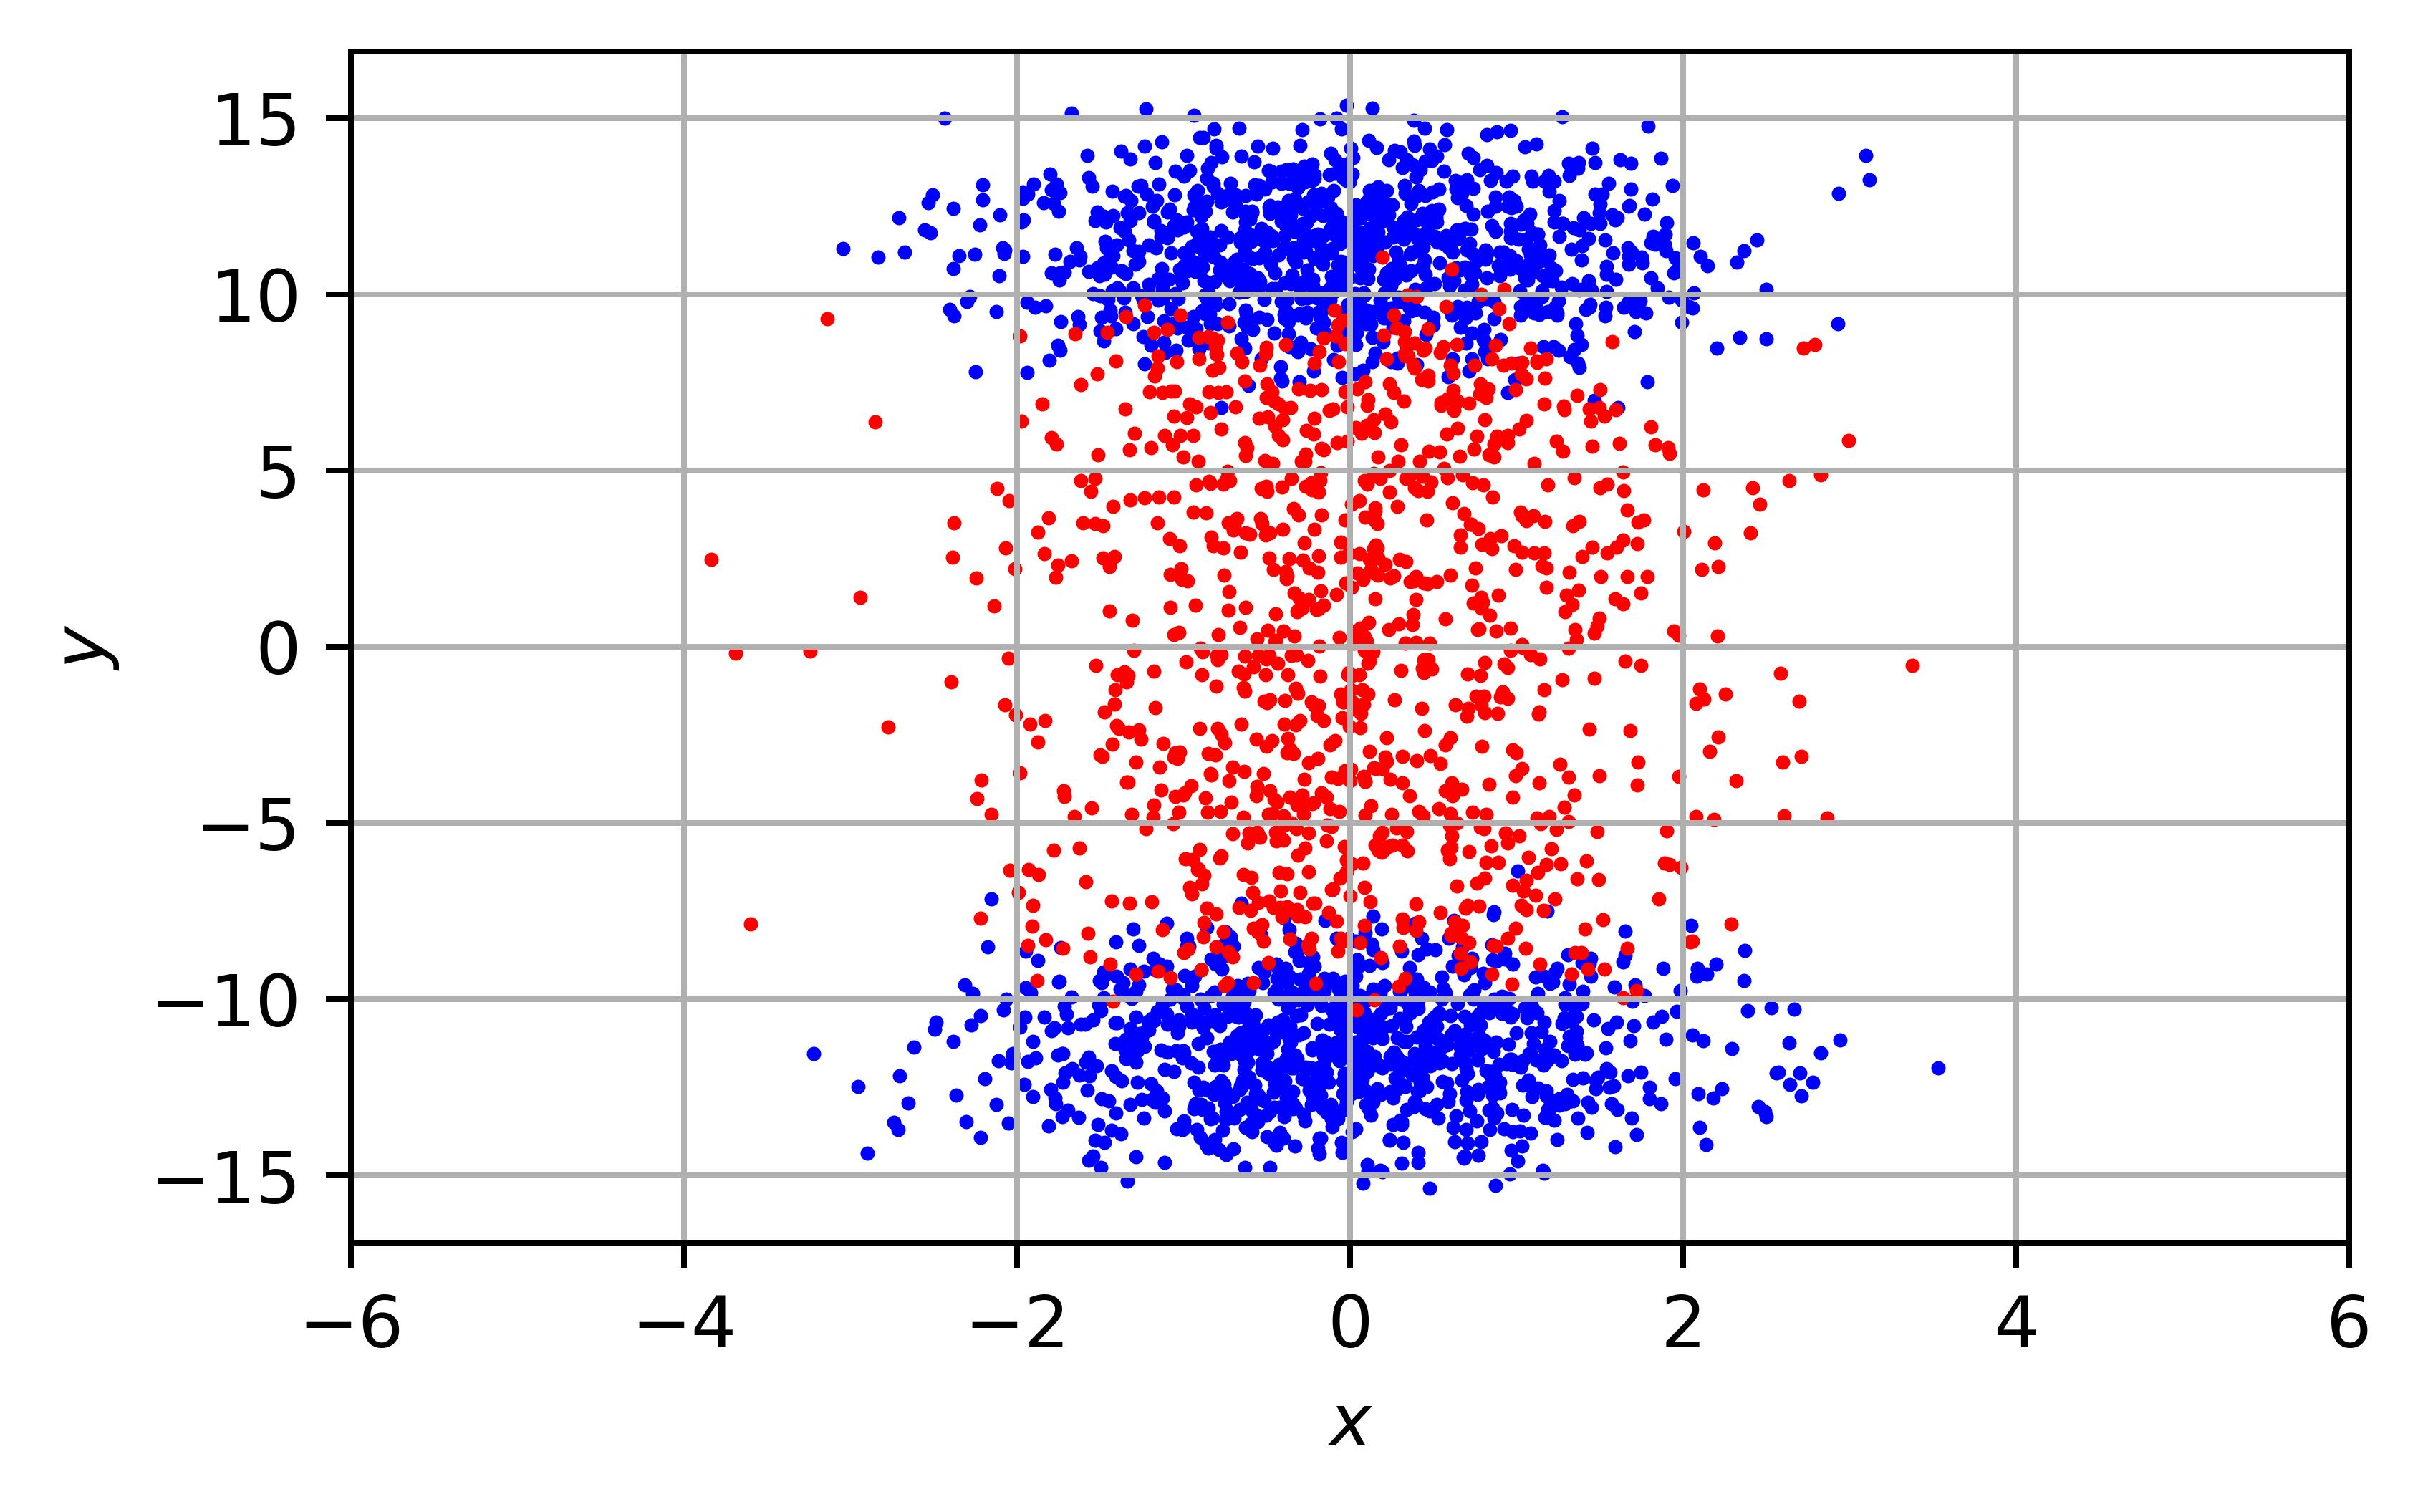
\includegraphics[width=0.4\textwidth]{./figure/Sample-Raising-1.jpg}
    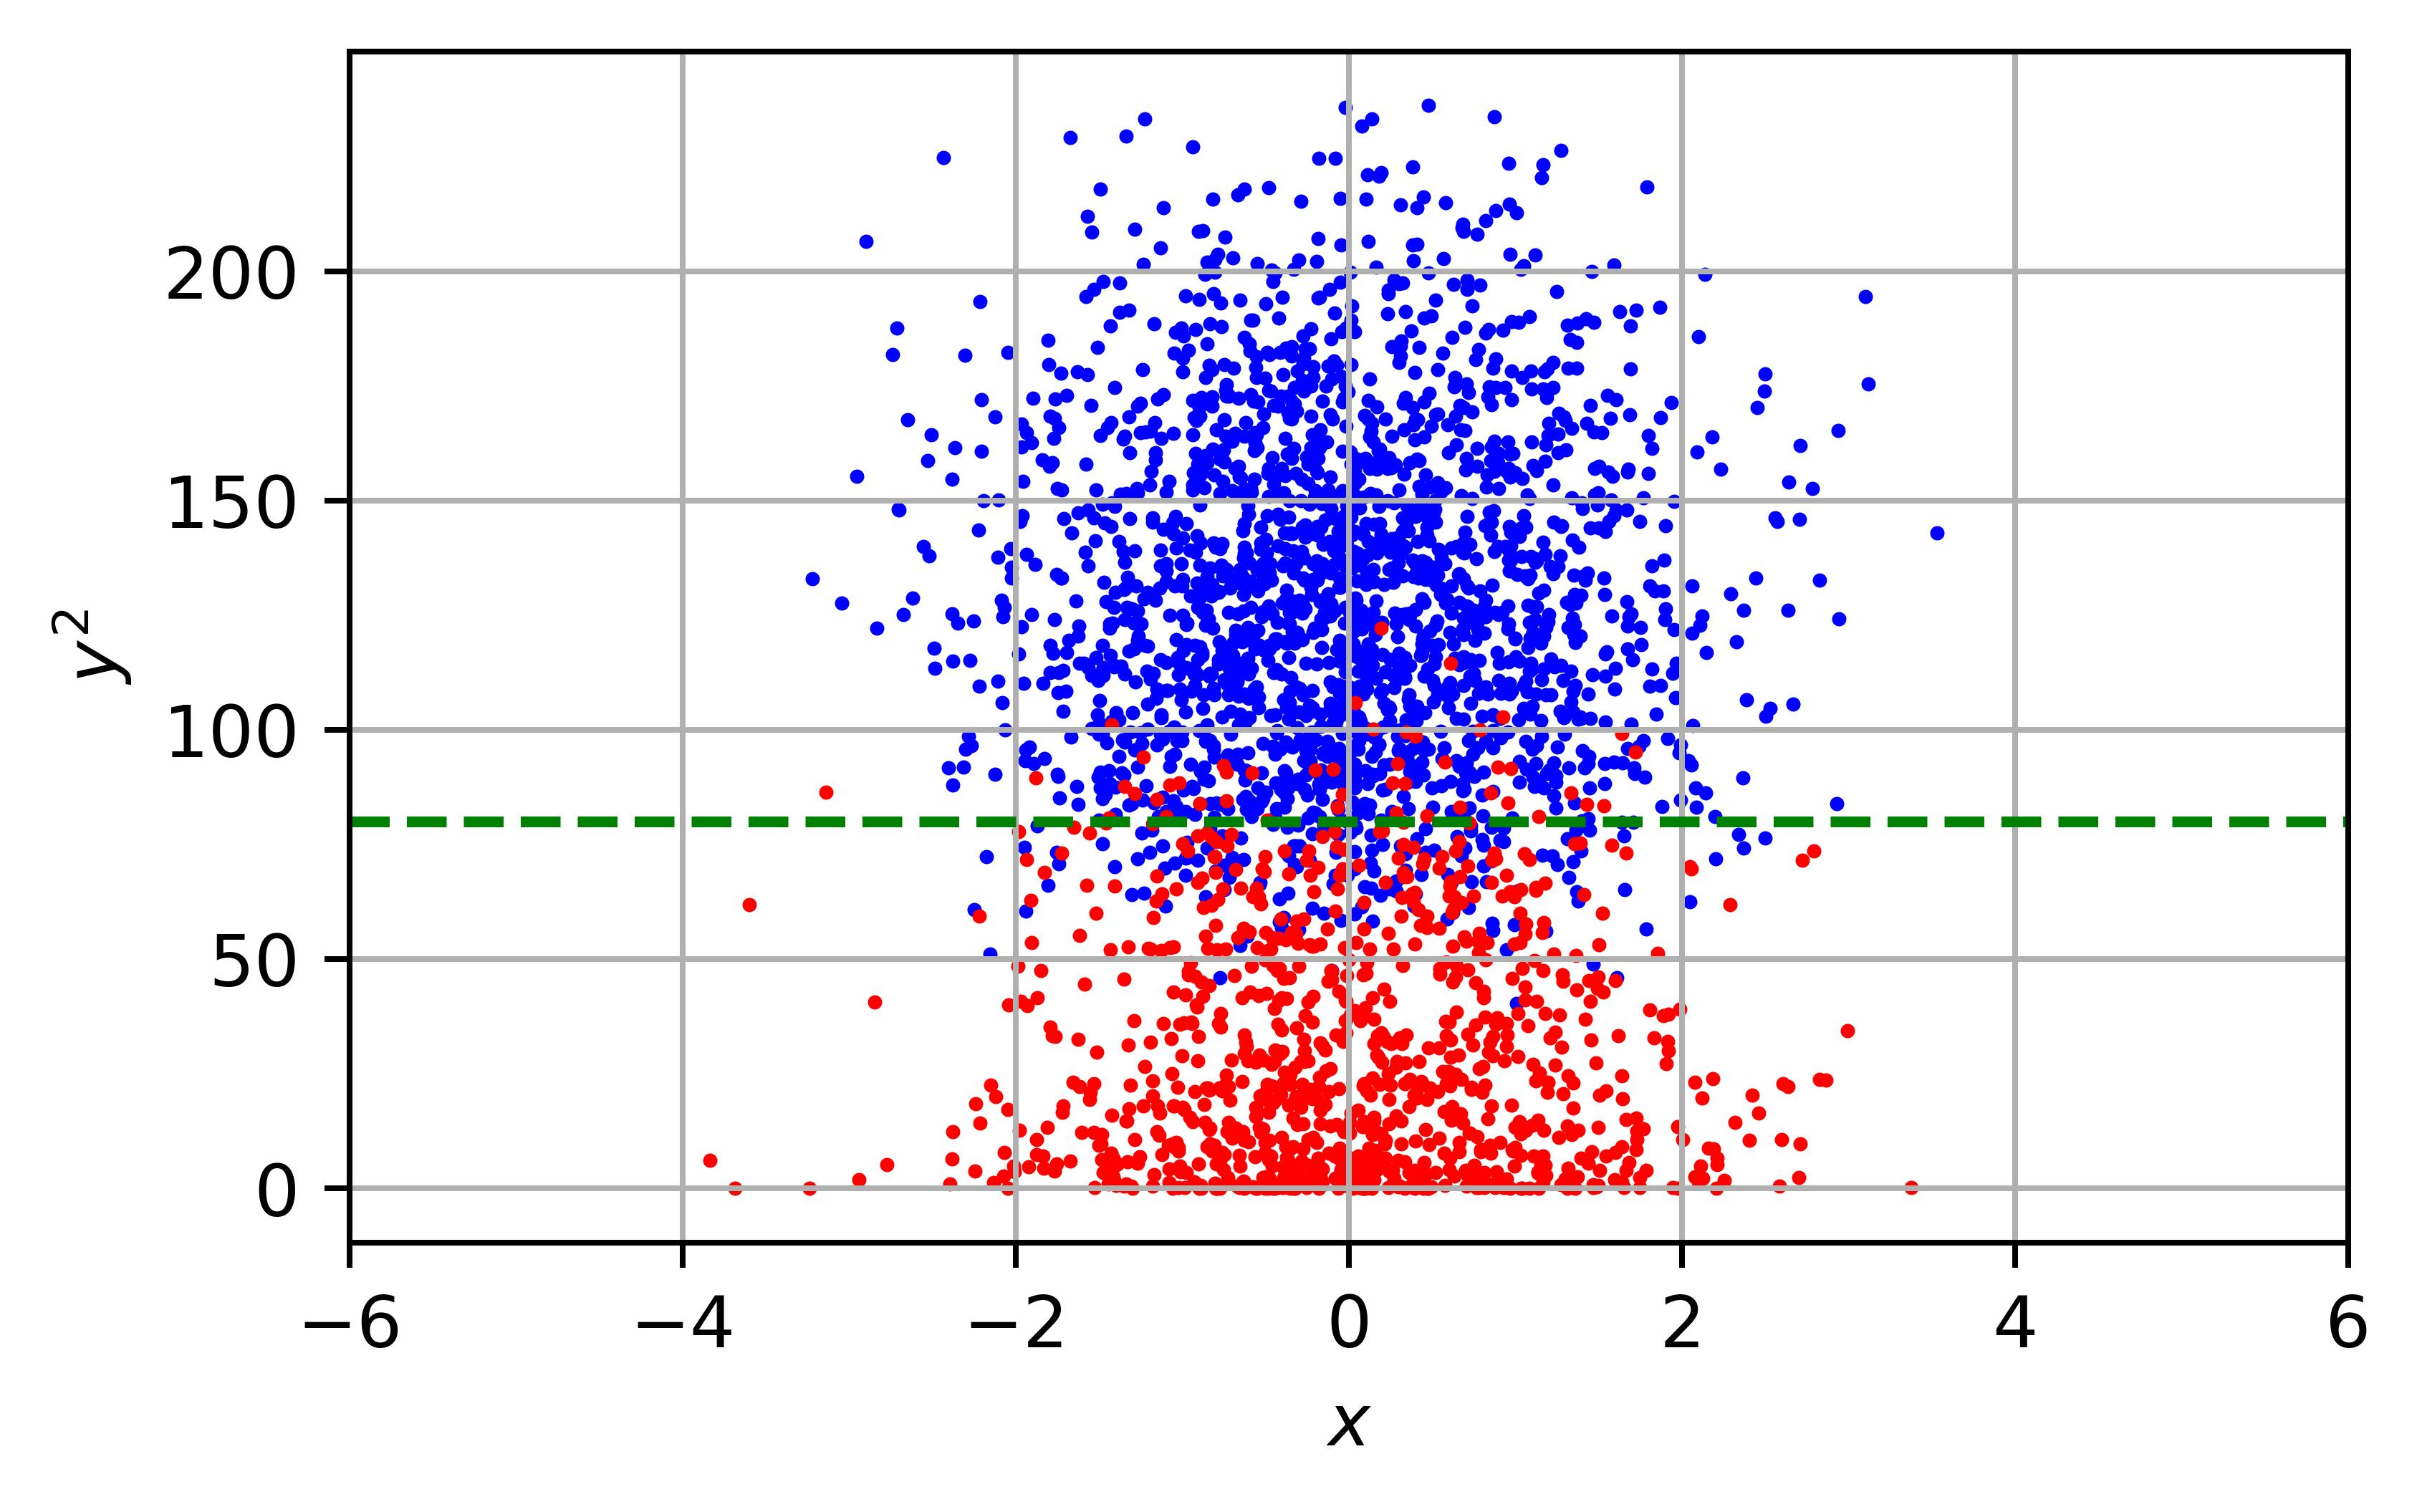
\includegraphics[width=0.4\textwidth]{./figure/Sample-Raising-2.jpg}
    \caption{Example for dimension raising. The left shows that origin data, where the data is not linearly separable, while the right shows the data after dimension raising, where the $y_2$ is easy to be separated by a line.}
  \end{figure}

\end{frame}

\section{Data Analysis}

\begin{frame}{Logistic regression}

  The logistic regression is a widely used linear classification model which: \vspace{.25cm}

  \begin{itemize}
    \item Will be less prone to overfitting; \vspace{.25cm}
    \item Can't catch the nonlinearity; \vspace{.25cm}
    \item Might be sensitive to the outliers; \vspace{.25cm}
    \item Can be easily expanded to categorical variables. \vspace{.25cm}
  \end{itemize}

\end{frame}

\begin{frame}{Decision tree}

  The decision tree is a decision support recursive partitioning structure which: \vspace{.25cm}

  \begin{itemize}
    \item Don't require normalization or standardization of data; \vspace{.25cm}
    \item Can handle both categorical and numerical data; \vspace{.25cm}
    \item Will be prone to overfitting and sensitive to the noise; \vspace{.25cm}
    \item Not suitable for large dataset. \vspace{.25cm}
  \end{itemize}

\end{frame}

\begin{frame}{Multilayer perceptron (MLP)}

  The multilayer perceptron (MLP) is a basic kind of neural network which: \vspace{.25cm}

  \begin{itemize}
    \item Can handle nonlinearity (or approximate any function); \vspace{.25cm}
    \item Can automatically extract features during training; \vspace{.25cm}
    \item Can handle large datasets; \vspace{.25cm}
    \item Will be sensitive to hyperparameters and noise. \vspace{.25cm}
  \end{itemize}

\end{frame}

\section{Solution}

\subsection{Solution - Task 1}

\begin{frame}{Task 1 - Overview}

  \begin{figure}
    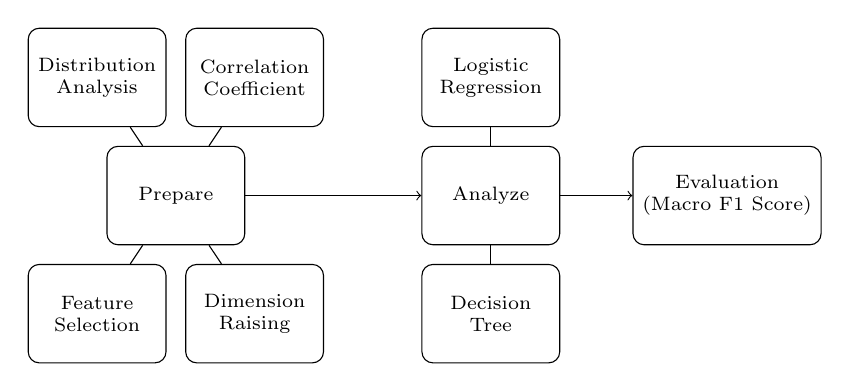
\begin{tikzpicture}[minimum width=1.75cm, minimum height=1.25cm, font=\scriptsize]
      \node[draw, align=center, rounded corners]  (P)   at ( 0,  0.0)    {Prepare};
      \node[draw, align=center, rounded corners]  (D)   at (-1,  1.5)    {Distribution \\ Analysis};
      \node[draw, align=center, rounded corners]  (C)   at ( 1,  1.5)    {Correlation \\ Coefficient};
      \node[draw, align=center, rounded corners]  (F)   at (-1, -1.5)    {Feature \\ Selection};
      \node[draw, align=center, rounded corners]  (R)   at ( 1, -1.5)    {Dimension \\ Raising};

      \node[draw, align=center, rounded corners]  (M)   at ( 4,  0.0)    {Analyze};
      \node[draw, align=center, rounded corners]  (LR)  at ( 4,  1.5)    {Logistic \\ Regression};
      \node[draw, align=center, rounded corners]  (DT)  at ( 4, -1.5)    {Decision \\ Tree};

      \node[draw, align=center, rounded corners]  (E)   at ( 7,  0.0)    {Evaluation \\ (Macro F1 Score)};

      \draw[->] (P) -- (M);

      \draw[-]  (P) -- (D);
      \draw[-]  (P) -- (C);
      \draw[-]  (P) -- (F);
      \draw[-]  (P) -- (R);

      \draw[-]  (M) -- (LR);
      \draw[-]  (M) -- (DT);

      \draw[->] (M) -- (E);
    \end{tikzpicture}
    \caption{Overview Flowchart.}
  \end{figure}

\end{frame}

\begin{frame}{Task 1 - Preformance - Logistic Regression}

  \begin{table}[H]
    \centering
    \begin{tabular}{|c|c|c|c|}
      \hline
      Penalty & \makecell{Dimension                         \\ Raising \\ (Degree)} & F1 Score & \makecell{Time/Mem \\ (s/MB)} \\
      \hline
      None    & None                & $0.7909$ & $1.55/735$ \\
      \hline
      None    & $2$                 & $0.7905$ & $1.41/730$ \\
      \hline
      None    & $3$                 & $0.7909$ & $1.28/741$ \\
      \hline
      Lasso   & None                & $0.7912$ & $1.66/736$ \\
      \hline
      Ridge   & None                & $0.7915$ & $1.65/735$ \\
      \hline
    \end{tabular}
    \caption{Preformance for logistic regression. We tested each option with $5$ times cross validation ($80\%$ for training set, $20\%$ for training set) and $1$ times that using all data as training set. The f1 scores showed in the table is the average f1 score for cross validation, the time is the total time for $6$ run, and the memory usage is tested using all the data as training set.}
  \end{table}

\end{frame}

\begin{frame}{Task 1 - Preformance - Decision Tree}

  \begin{table}[H]
    \centering
    \begin{tabular}{|c|c|c|c|c|}
      \hline
      Max Depth & \makecell{Number of                                   \\ Threshold} & Criterion & F1 Score & \makecell{Time/Mem \\ (s/MB)}               \\
      \hline
      $10$      & $64$                & gini    & $0.7502$ & $17.5/497$ \\
      \hline
      $10$      & $128$               & gini    & $0.7485$ & $16.4/498$ \\
      \hline
      $12$      & $64$                & gini    & $0.7266$ & $25.2/497$ \\
      \hline
      $10$      & $64$                & entropy & $0.7428$ & $16.4/501$ \\
      \hline
    \end{tabular}
    \caption{Preformance for decision tree. We tested each option with $5$ times cross validation ($80\%$ for training set, $20\%$ for training set) and $1$ times that using all data as training set. The f1 scores showed in the table is the average f1 score for cross validation, the time is the total time for $6$ run, and the memory usage is tested using all the data as training set.}
  \end{table}

\end{frame}

\subsection{Solution - Task 2}

\begin{frame}{Task 2 - Overview}

  \begin{figure}
    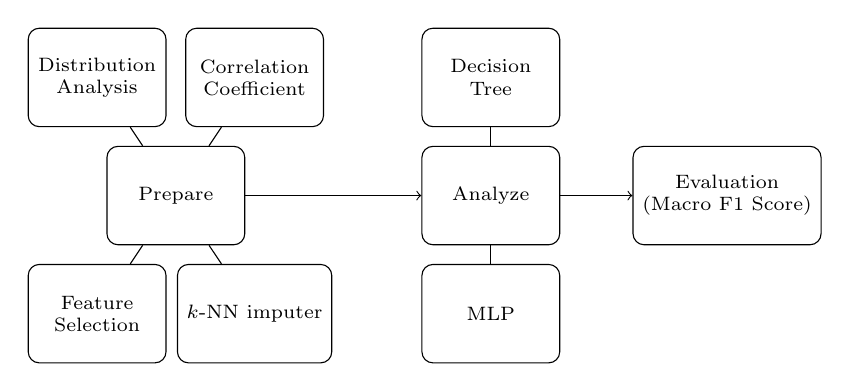
\begin{tikzpicture}[minimum width=1.75cm, minimum height=1.25cm, font=\scriptsize]
      \node[draw, align=center, rounded corners]  (P)   at ( 0,  0.0)    {Prepare};
      \node[draw, align=center, rounded corners]  (D)   at (-1,  1.5)    {Distribution \\ Analysis};
      \node[draw, align=center, rounded corners]  (C)   at ( 1,  1.5)    {Correlation \\ Coefficient};
      \node[draw, align=center, rounded corners]  (F)   at (-1, -1.5)    {Feature \\ Selection};
      \node[draw, align=center, rounded corners]  (KNN) at ( 1, -1.5)    {$k$-NN imputer};

      \node[draw, align=center, rounded corners]  (M)   at ( 4,  0.0)    {Analyze};
      \node[draw, align=center, rounded corners]  (DT)  at ( 4,  1.5)    {Decision \\ Tree};
      \node[draw, align=center, rounded corners]  (MLP) at ( 4, -1.5)    {MLP};

      \node[draw, align=center, rounded corners]  (E)   at ( 7,  0.0)    {Evaluation \\ (Macro F1 Score)};

      \draw[->] (P) -- (M);

      \draw[-]  (P) -- (D);
      \draw[-]  (P) -- (C);
      \draw[-]  (P) -- (F);
      \draw[-]  (P) -- (KNN);

      \draw[-]  (M) -- (DT);
      \draw[-]  (M) -- (MLP);

      \draw[->] (M) -- (E);
    \end{tikzpicture}
    \caption{Overview Flowchart.}
  \end{figure}

\end{frame}

\begin{frame}{Task 2 - Distribution Analysis}

  \begin{figure}[H]
    \centering
    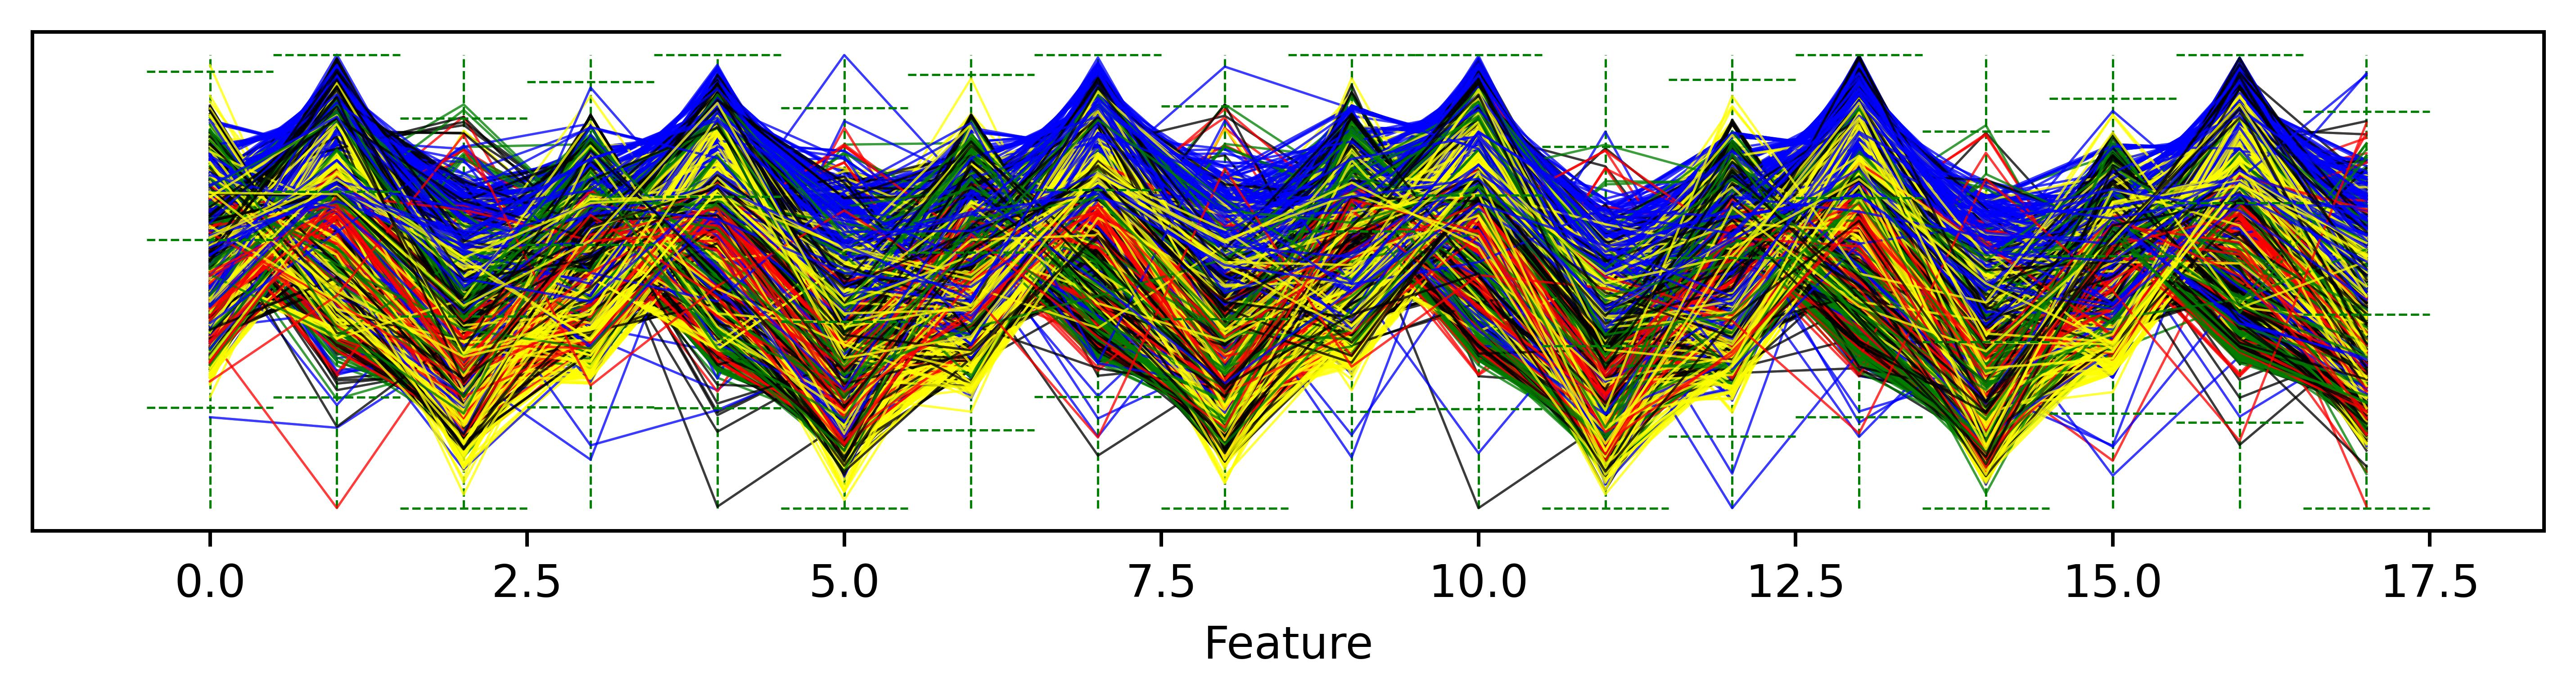
\includegraphics[width=0.9\textwidth]{../code/Task2/Analysis/PC.jpg} \\
    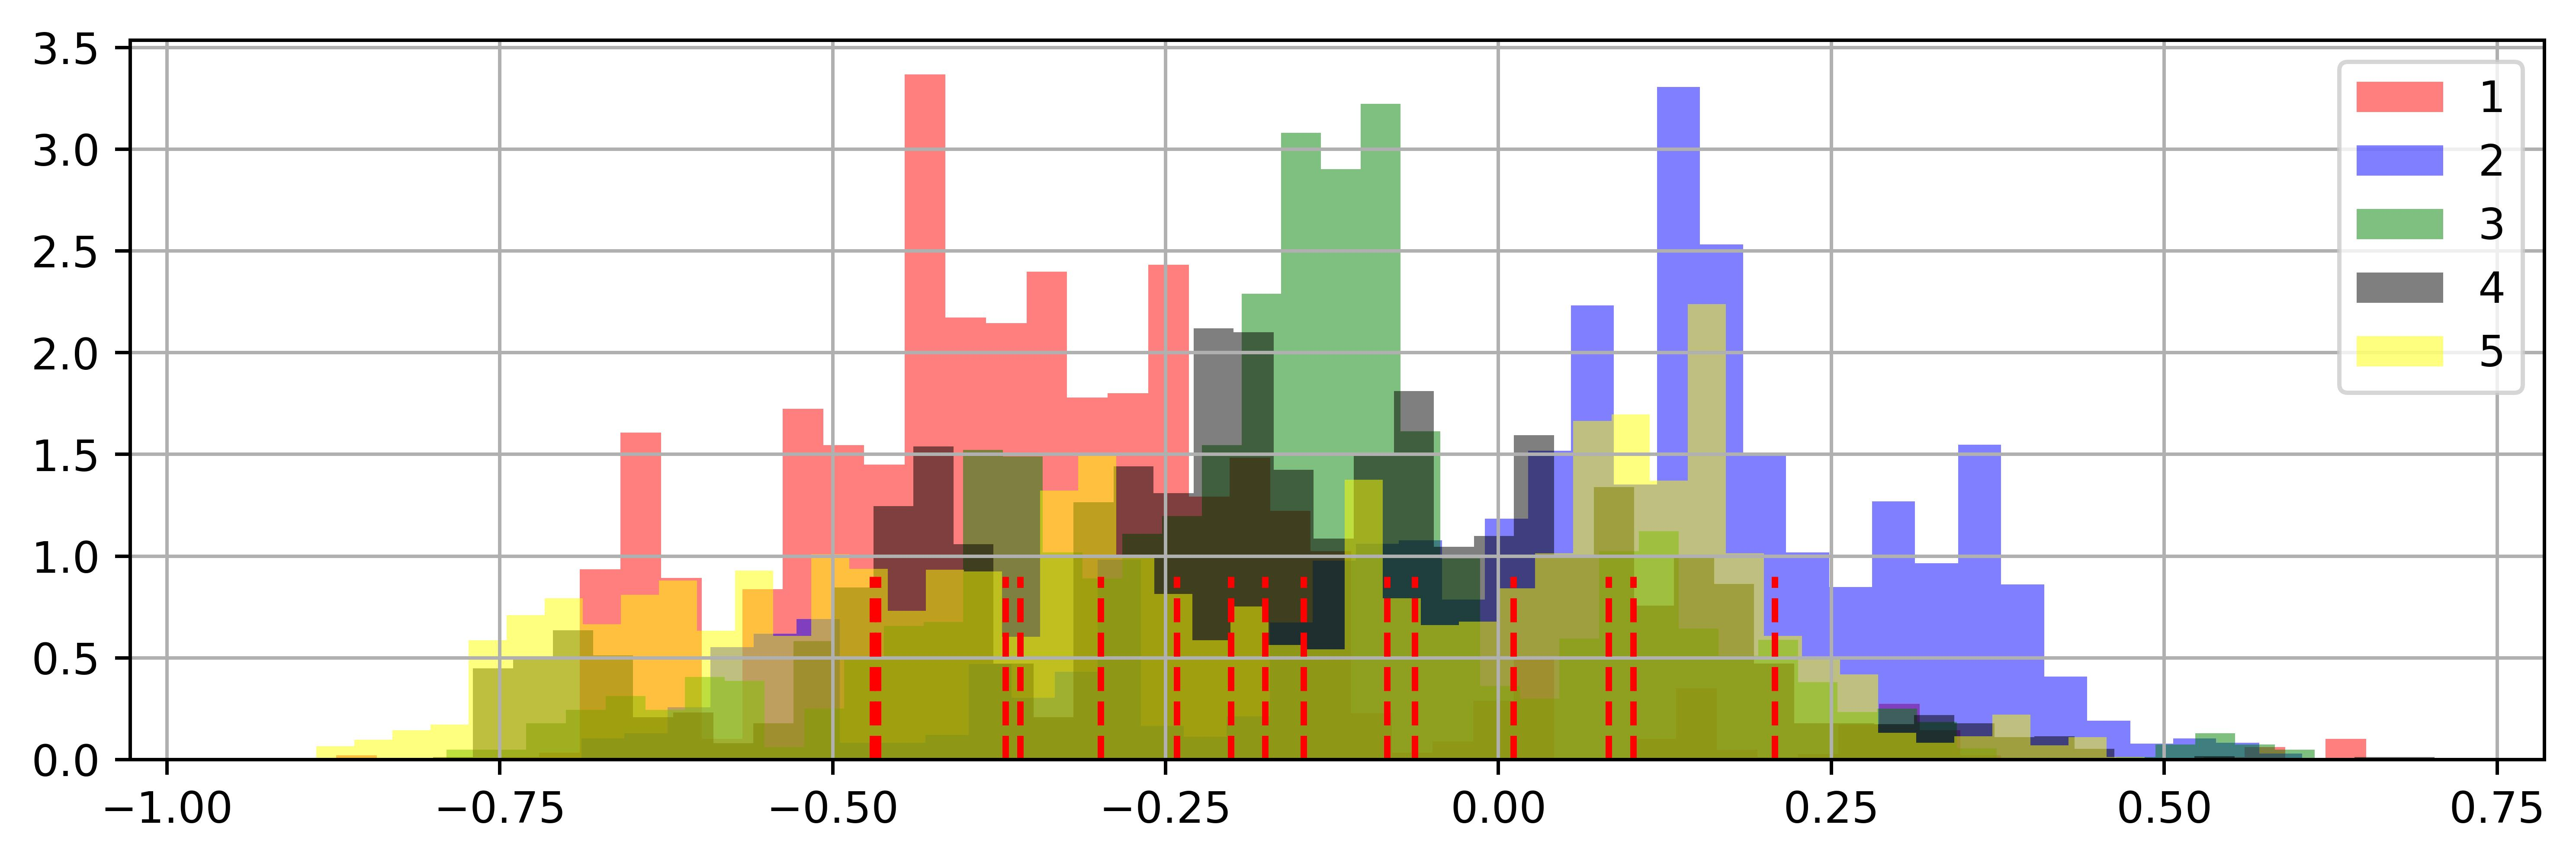
\includegraphics[width=0.3\textwidth]{../code/Task2/Analysis/Hist-2.jpg}
    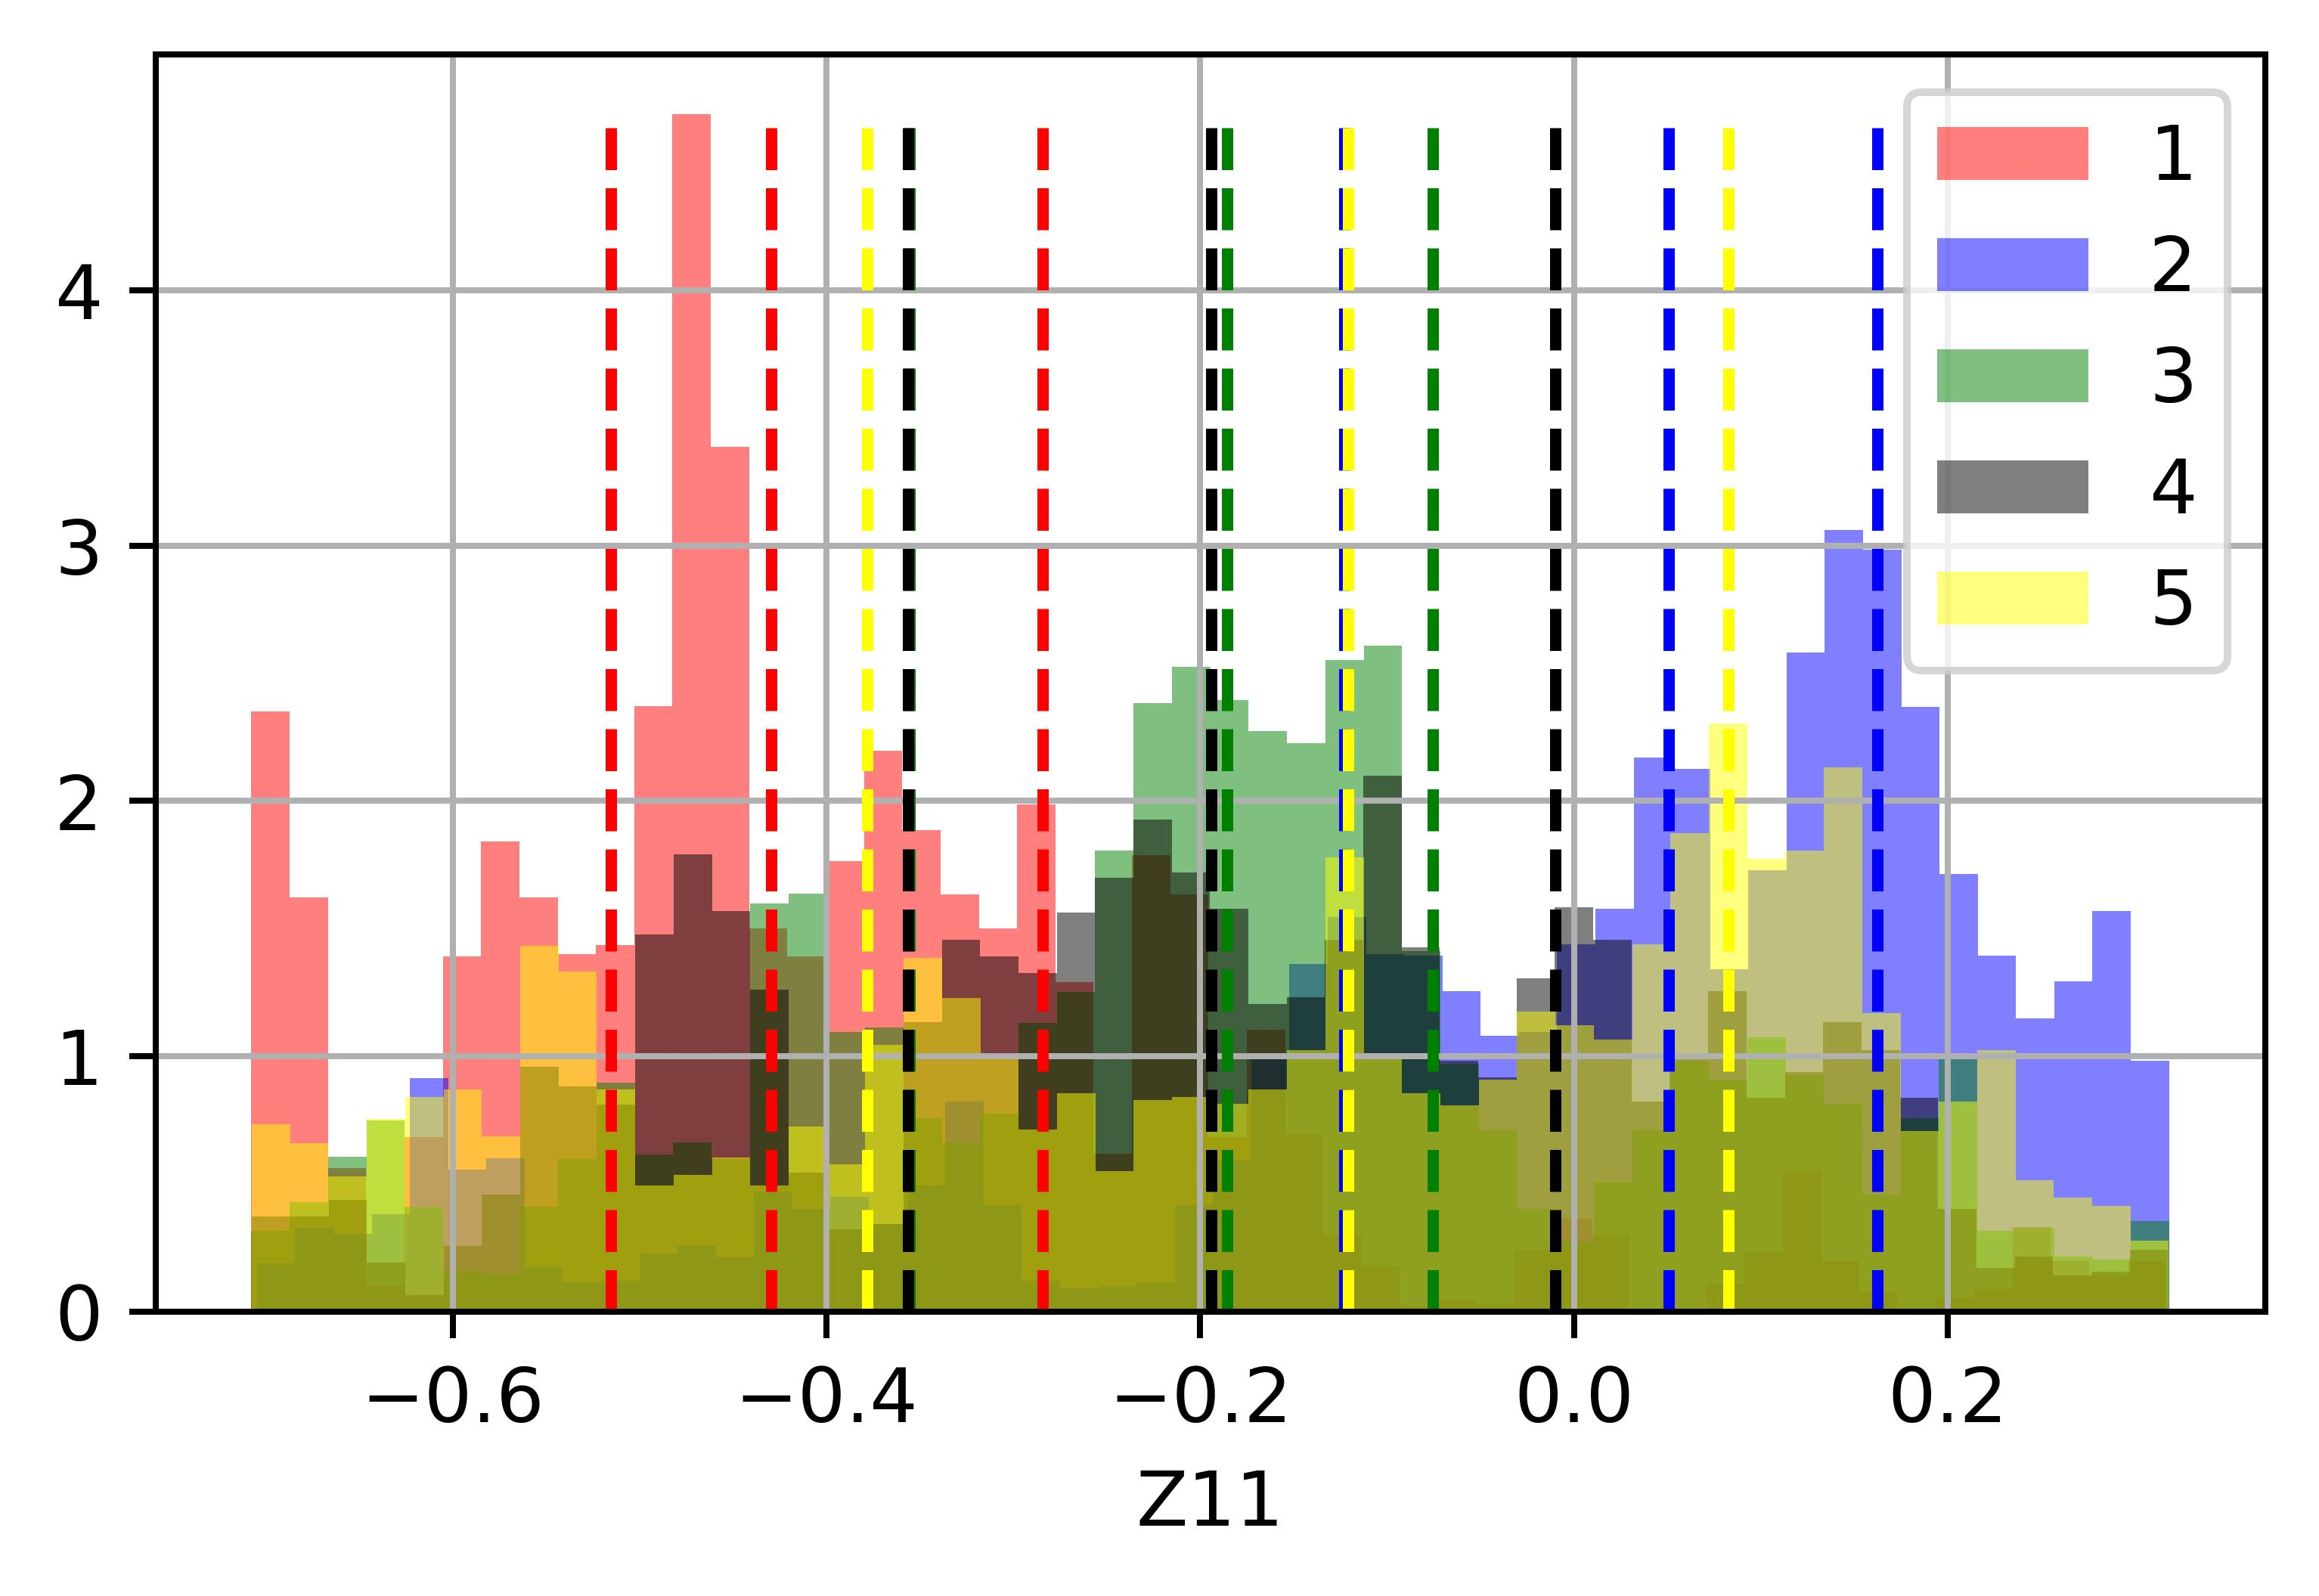
\includegraphics[width=0.3\textwidth]{../code/Task2/Analysis/Hist-5.jpg}
    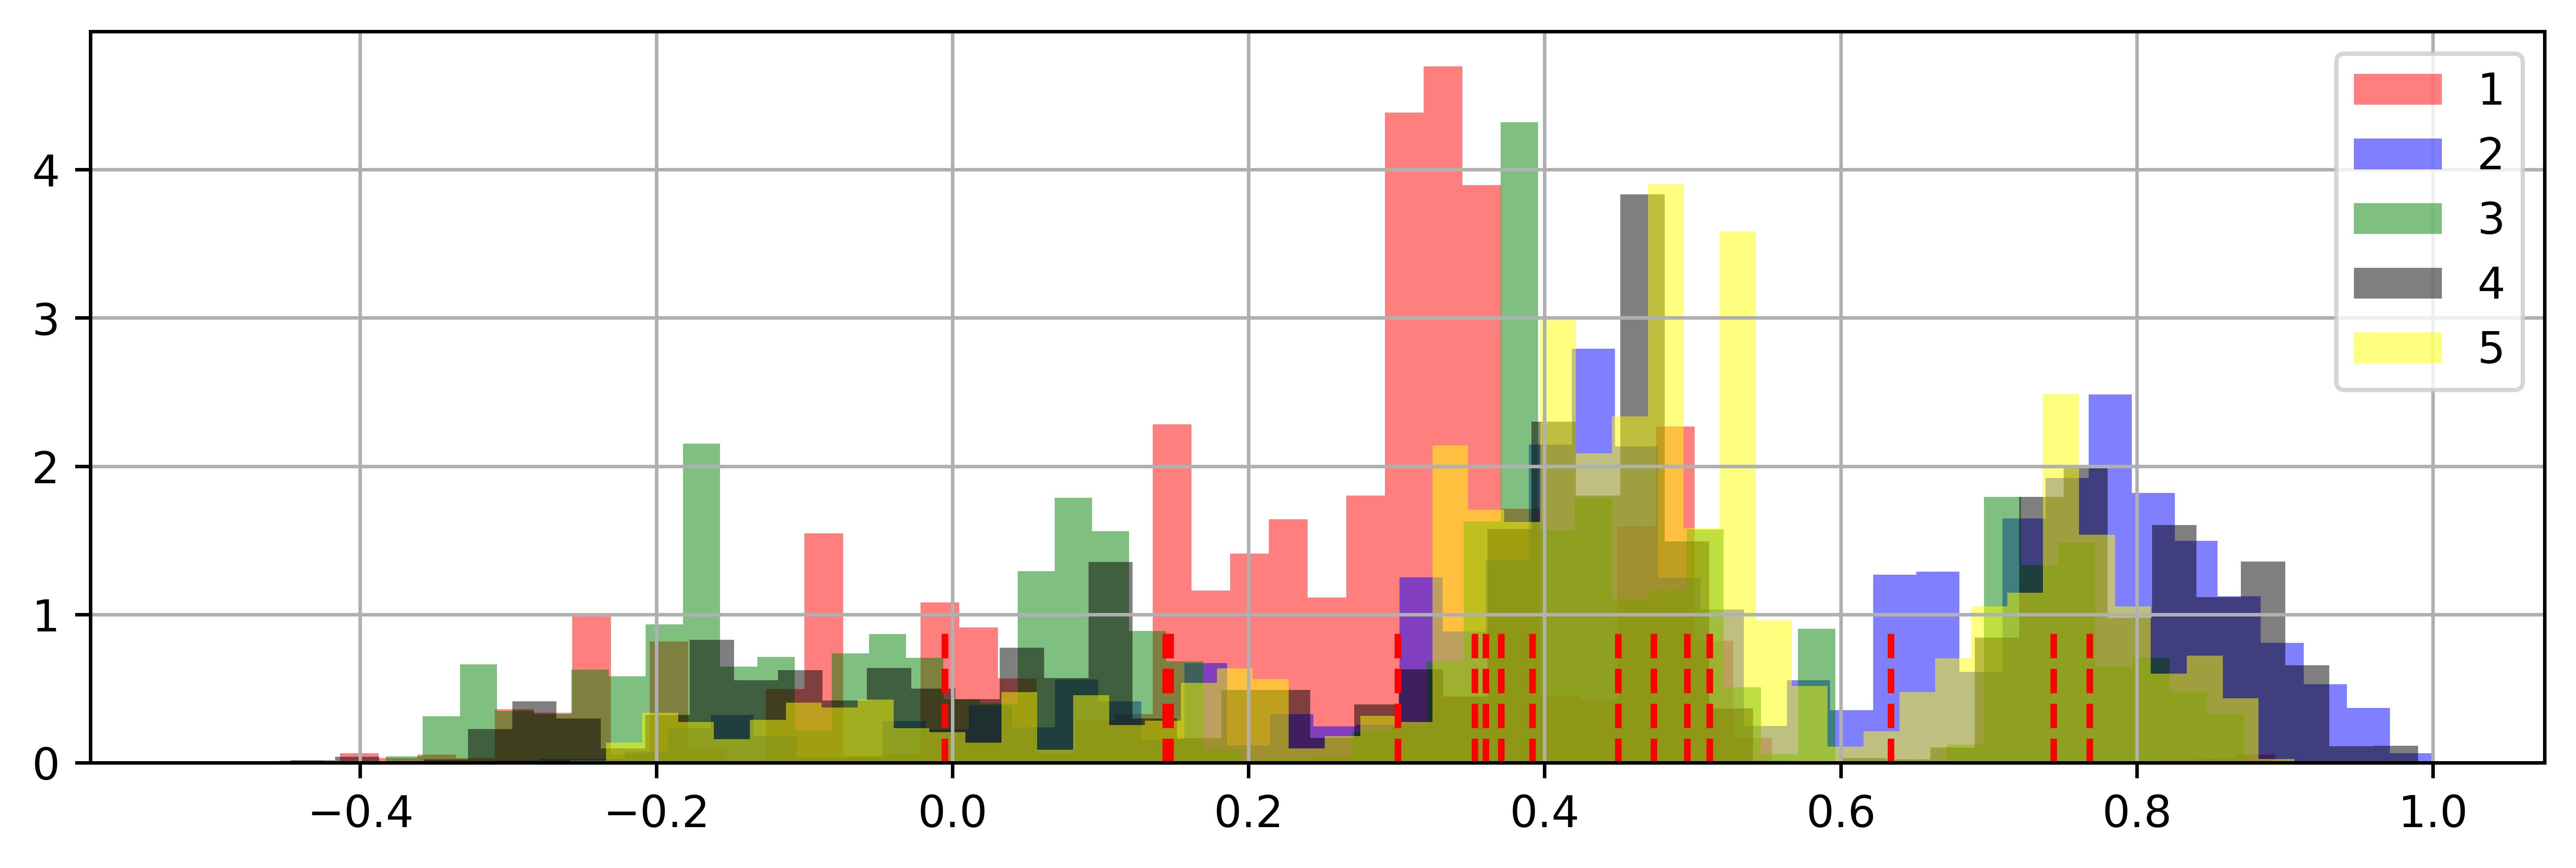
\includegraphics[width=0.3\textwidth]{../code/Task2/Analysis/Hist-7.jpg}
    \caption{Data visualization for task 2. The top shows the parallel coordinate plot for each features (we chose $10\%$ of total data), and the below shows even the features can't be easily separated, but the distribution of the labels can be differnet (the top and bottom $5\%$ points are considered as outliers, and will not be shown).}
  \end{figure}

\end{frame}

\begin{frame}{Task 2 - Correlation Coefficient}

  \begin{figure}[H]
    \centering
    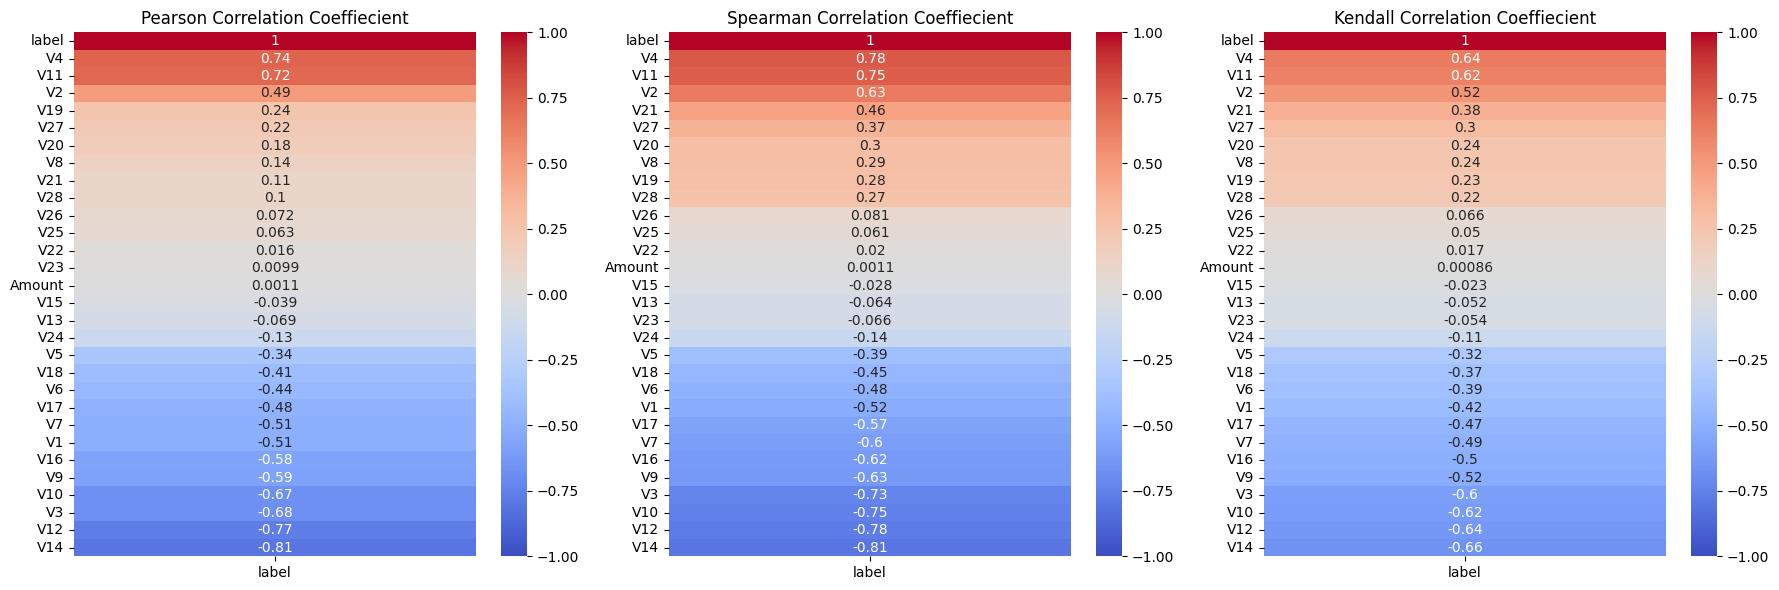
\includegraphics[width=\textwidth]{../code/Task3/Analysis/corrcoef.jpg} \\
    \caption{Correlation coefficient for each features.}
  \end{figure}

  We droped the features with all the correlation coefficient less than a threshold (e.g. 0.1).

\end{frame}

\begin{frame}{Task 2 - Preformance - Decision Tree}

  \begin{table}[H]
    \centering
    \begin{tabular}{|c|c|c|c|c|c|}
      \hline
      \makecell{Max                                           \\Depth} & \makecell{Num of                                                          \\ Threshold} & Criterion & \makecell{Feature \\ Selection}& F1 Score & \makecell{Time/Mem \\ (s/MB)}               \\
      \hline
      $10$ & $64$  & gini    & False & $0.8097$ & $153.6/606$ \\
      \hline
      $10$ & $128$ & gini    & False & $0.8043$ & $168.5/650$ \\
      \hline
      $12$ & $64$  & gini    & False & $0.8511$ & $172.8/601$ \\
      \hline
      $10$ & $64$  & entropy & False & $0.8184$ & $147.7/608$ \\
      \hline
      $10$ & $64$  & gini    & True  & $0.8052$ & $80.7/585$  \\
      \hline
    \end{tabular}
    \caption{Preformance for decision tree. We tested each option with $5$ times cross validation ($80\%$ for training set, $20\%$ for training set) and $1$ times that using all data as training set. The f1 scores showed in the table is the average f1 score for cross validation, the time is the total time for $6$ run, and the memory usage is tested using all the data as training set.}
  \end{table}

\end{frame}

\begin{frame}{Task 2 - Preformance - MLP}

  \begin{table}[H]
    \centering
    \begin{tabular}{|c|c|c|c|c|c|}
      \hline
      Dropout & Hidden Size & \makecell{Feature                                 \\ Selection} &Batch Size & F1 Score & \makecell{Time/Mem \\ (s/MB)} \\
      \hline
      $0.3$   & $128$       & False             & 512  & $0.9617$ & $219.4/856$ \\
      \hline
      $0.3$   & $64$        & False             & 512  & $0.9173$ & $212.9/812$ \\
      \hline
      $0.3$   & $256$       & False             & 512  & $0.9767$ & $221.7/856$ \\
      \hline
      $0.3$   & $128$       & False             & 1024 & $0.9629$ & $148.6/857$ \\
      \hline
      $0.3$   & $128$       & False             & 512  & $0.9644$ & $381.4/859$ \\
      \hline
      $0.3$   & $128$       & True              & 512  & $0.9474$ & $171.7/848$ \\
      \hline
    \end{tabular}
    \caption{Preformance for MLP. We tested each option with $5$ times cross validation ($80\%$ for training set, $20\%$ for training set) and $1$ times that using all data as training set. The f1 scores showed in the table is the average f1 score for cross validation, the time is the total time for $6$ run, and the memory usage is tested using all the data as training set.}
  \end{table}

\end{frame}

\subsection{Solution - Task 3}

\begin{frame}{Task 3 - Overview}

  \begin{figure}
    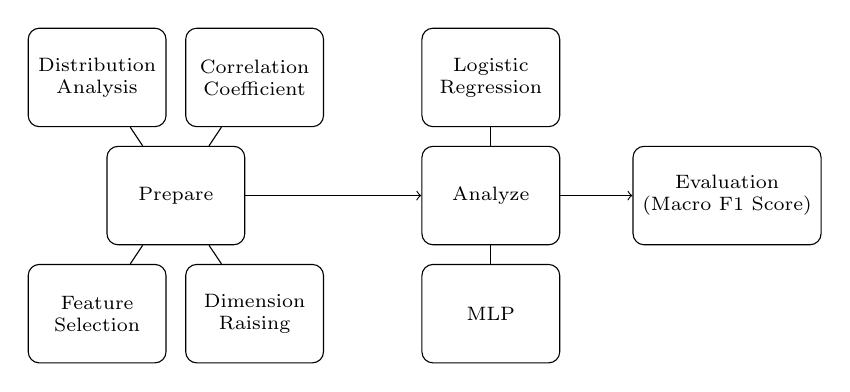
\begin{tikzpicture}[minimum width=1.75cm, minimum height=1.25cm, font=\scriptsize]
      \node[draw, align=center, rounded corners]  (P)   at ( 0,  0.0)    {Prepare};
      \node[draw, align=center, rounded corners]  (D)   at (-1,  1.5)    {Distribution \\ Analysis};
      \node[draw, align=center, rounded corners]  (C)   at ( 1,  1.5)    {Correlation \\ Coefficient};
      \node[draw, align=center, rounded corners]  (F)   at (-1, -1.5)    {Feature \\ Selection};
      \node[draw, align=center, rounded corners]  (R)   at ( 1, -1.5)    {Dimension \\ Raising};

      \node[draw, align=center, rounded corners]  (M)   at ( 4,  0.0)    {Analyze};
      \node[draw, align=center, rounded corners]  (LR)  at ( 4,  1.5)    {Logistic \\ Regression};
      \node[draw, align=center, rounded corners]  (MLP) at ( 4, -1.5)    {MLP};

      \node[draw, align=center, rounded corners]  (E)   at ( 7,  0.0)    {Evaluation \\ (Macro F1 Score)};

      \draw[->] (P) -- (M);

      \draw[-]  (P) -- (D);
      \draw[-]  (P) -- (C);
      \draw[-]  (P) -- (F);
      \draw[-]  (P) -- (R);

      \draw[-]  (M) -- (LR);
      \draw[-]  (M) -- (MLP);

      \draw[->] (M) -- (E);
    \end{tikzpicture}
    \caption{Overview Flowchart.}
  \end{figure}

\end{frame}

\begin{frame}{Task 3 - Distribution Analysis}

  \begin{figure}[H]
    \centering
    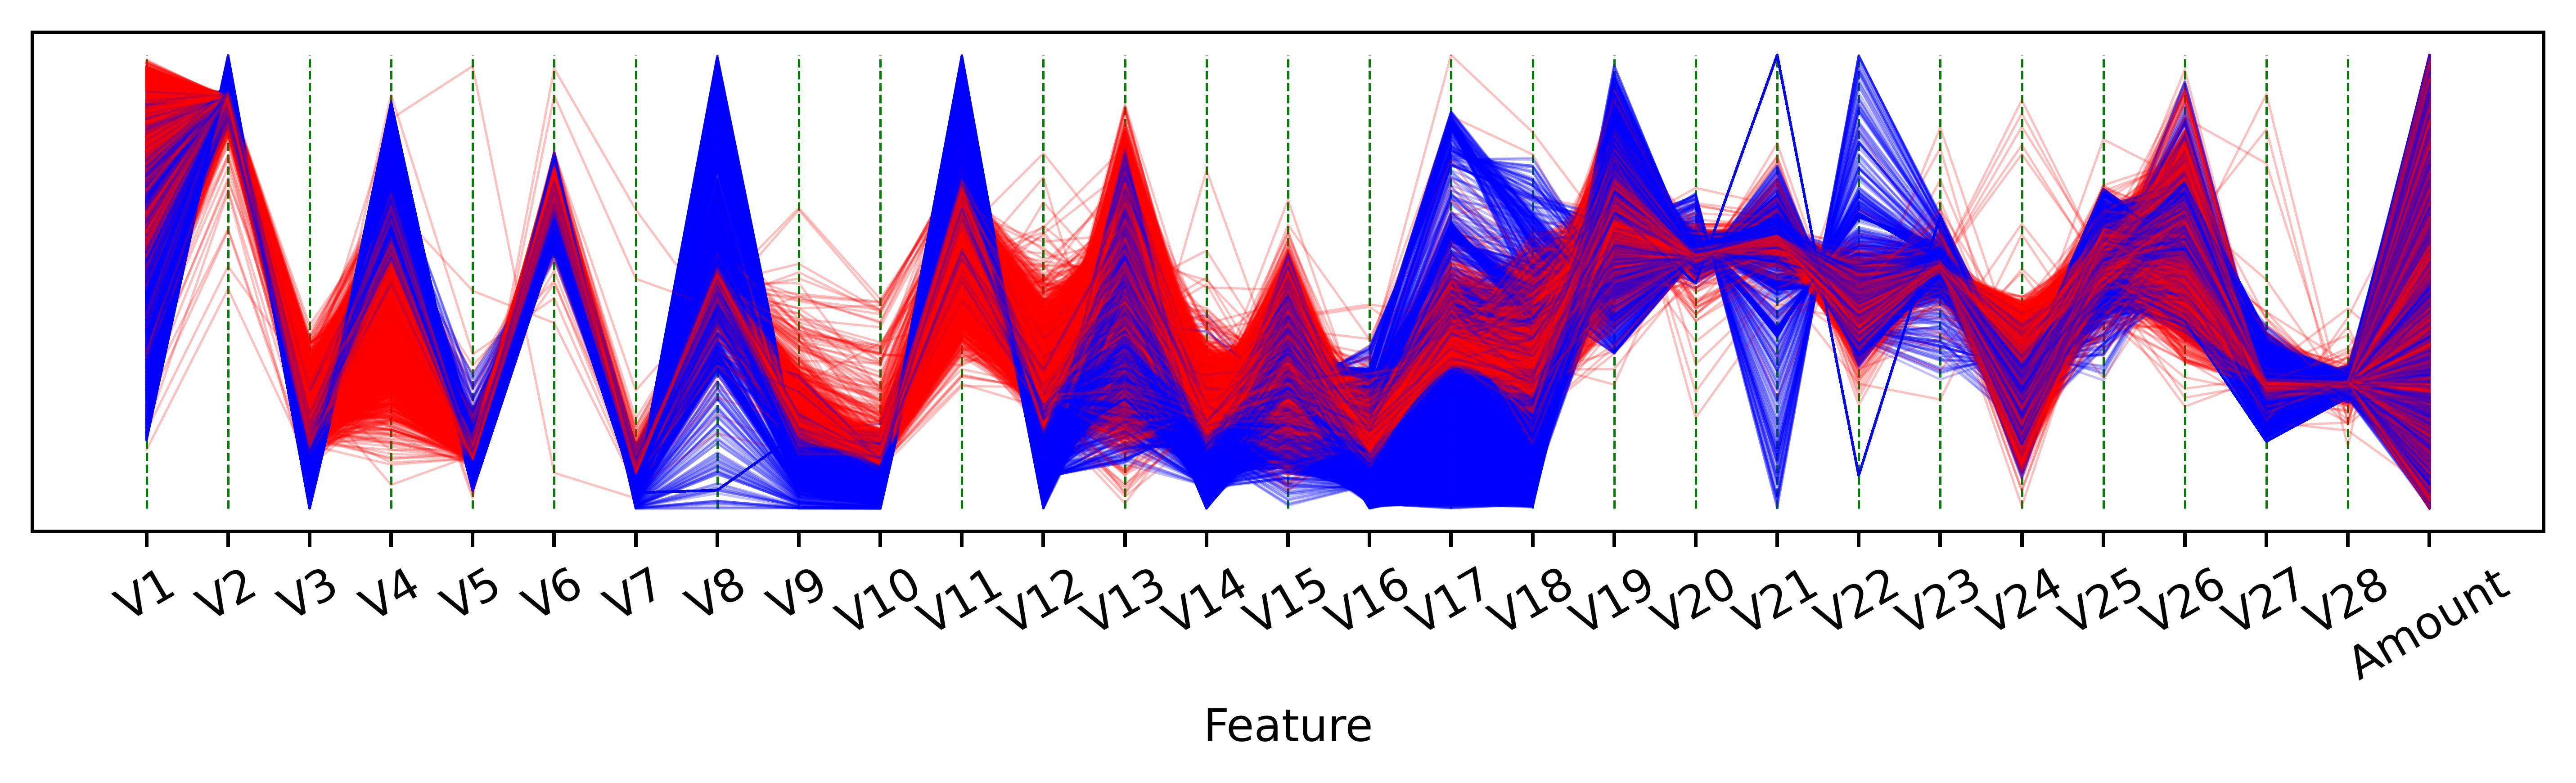
\includegraphics[width=0.9\textwidth]{../code/Task3/Analysis/PC.jpg} \\
    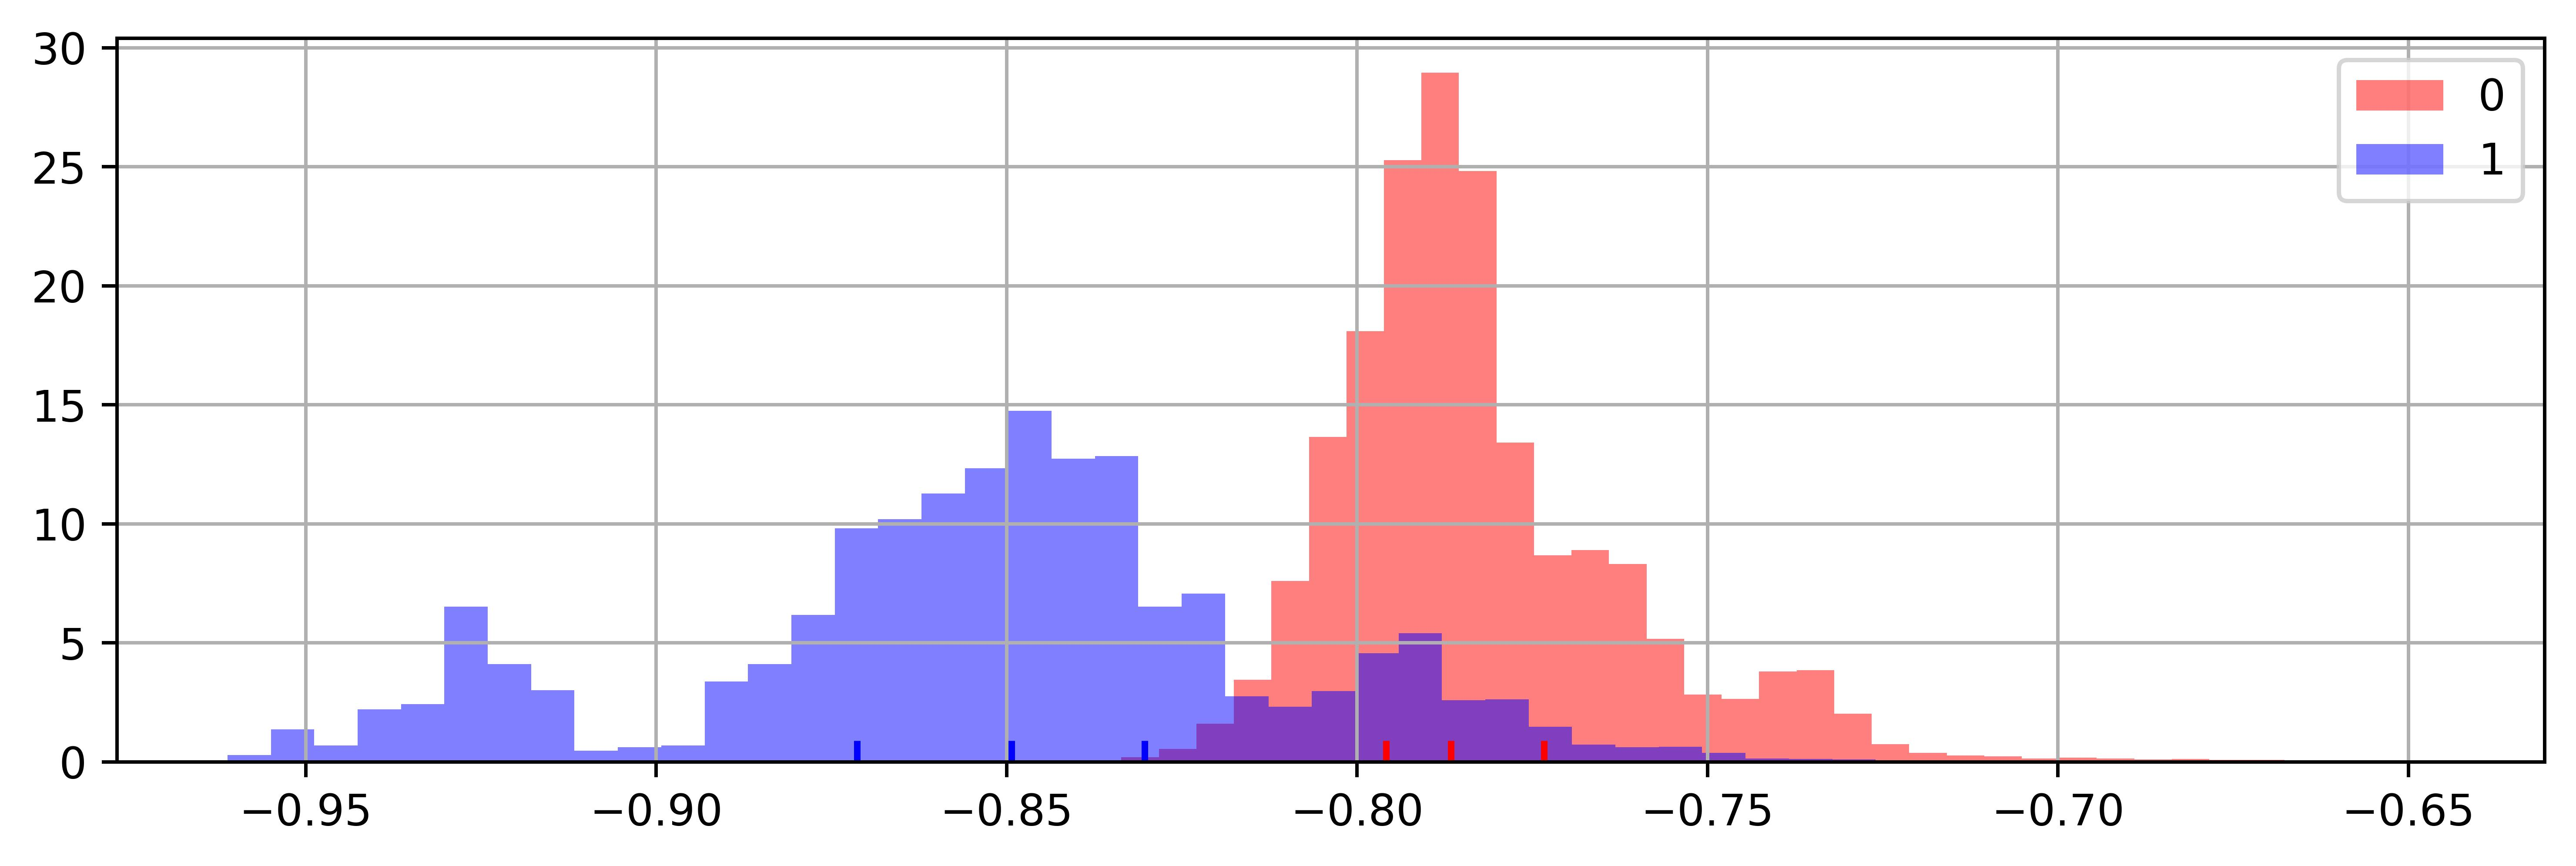
\includegraphics[width=0.3\textwidth]{../code/Task3/Analysis/Hist-9.jpg}
    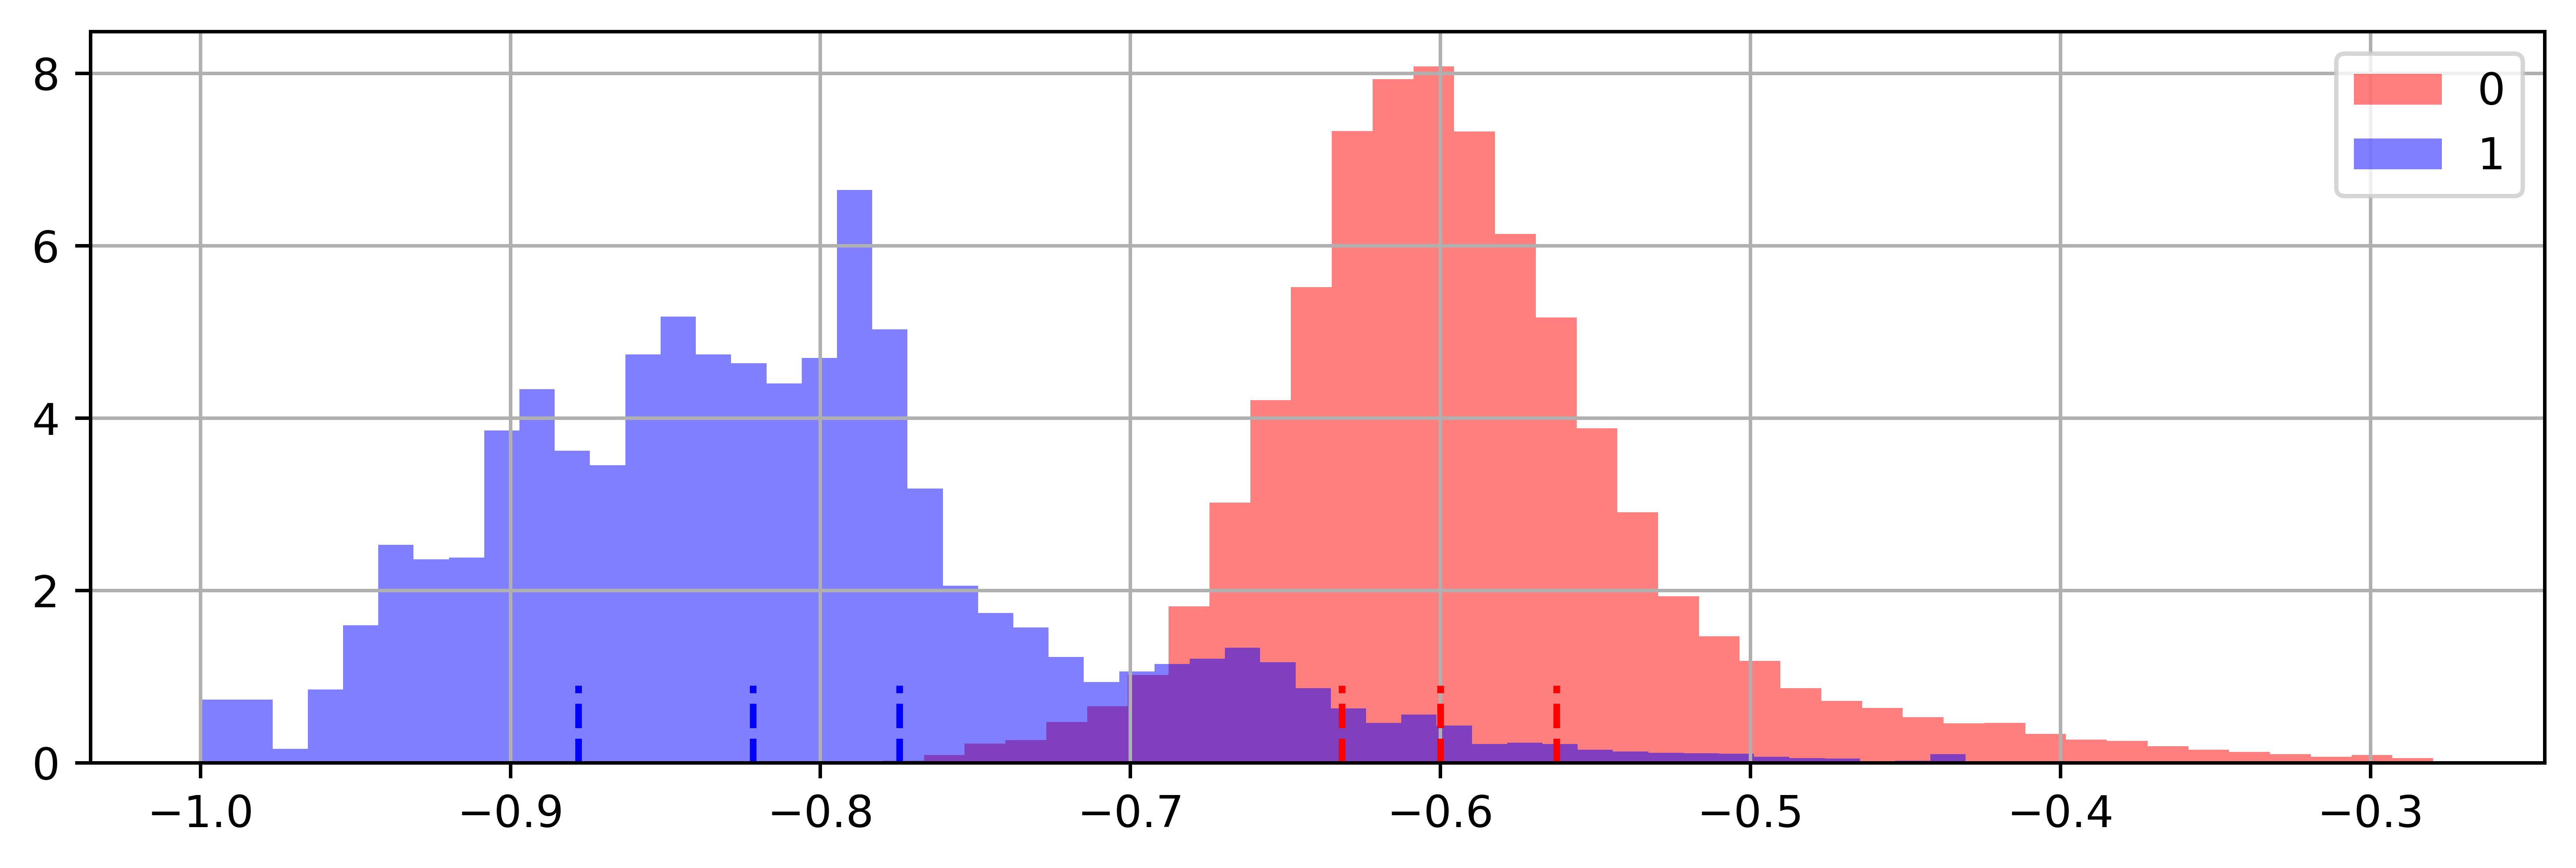
\includegraphics[width=0.3\textwidth]{../code/Task3/Analysis/Hist-13.jpg}
    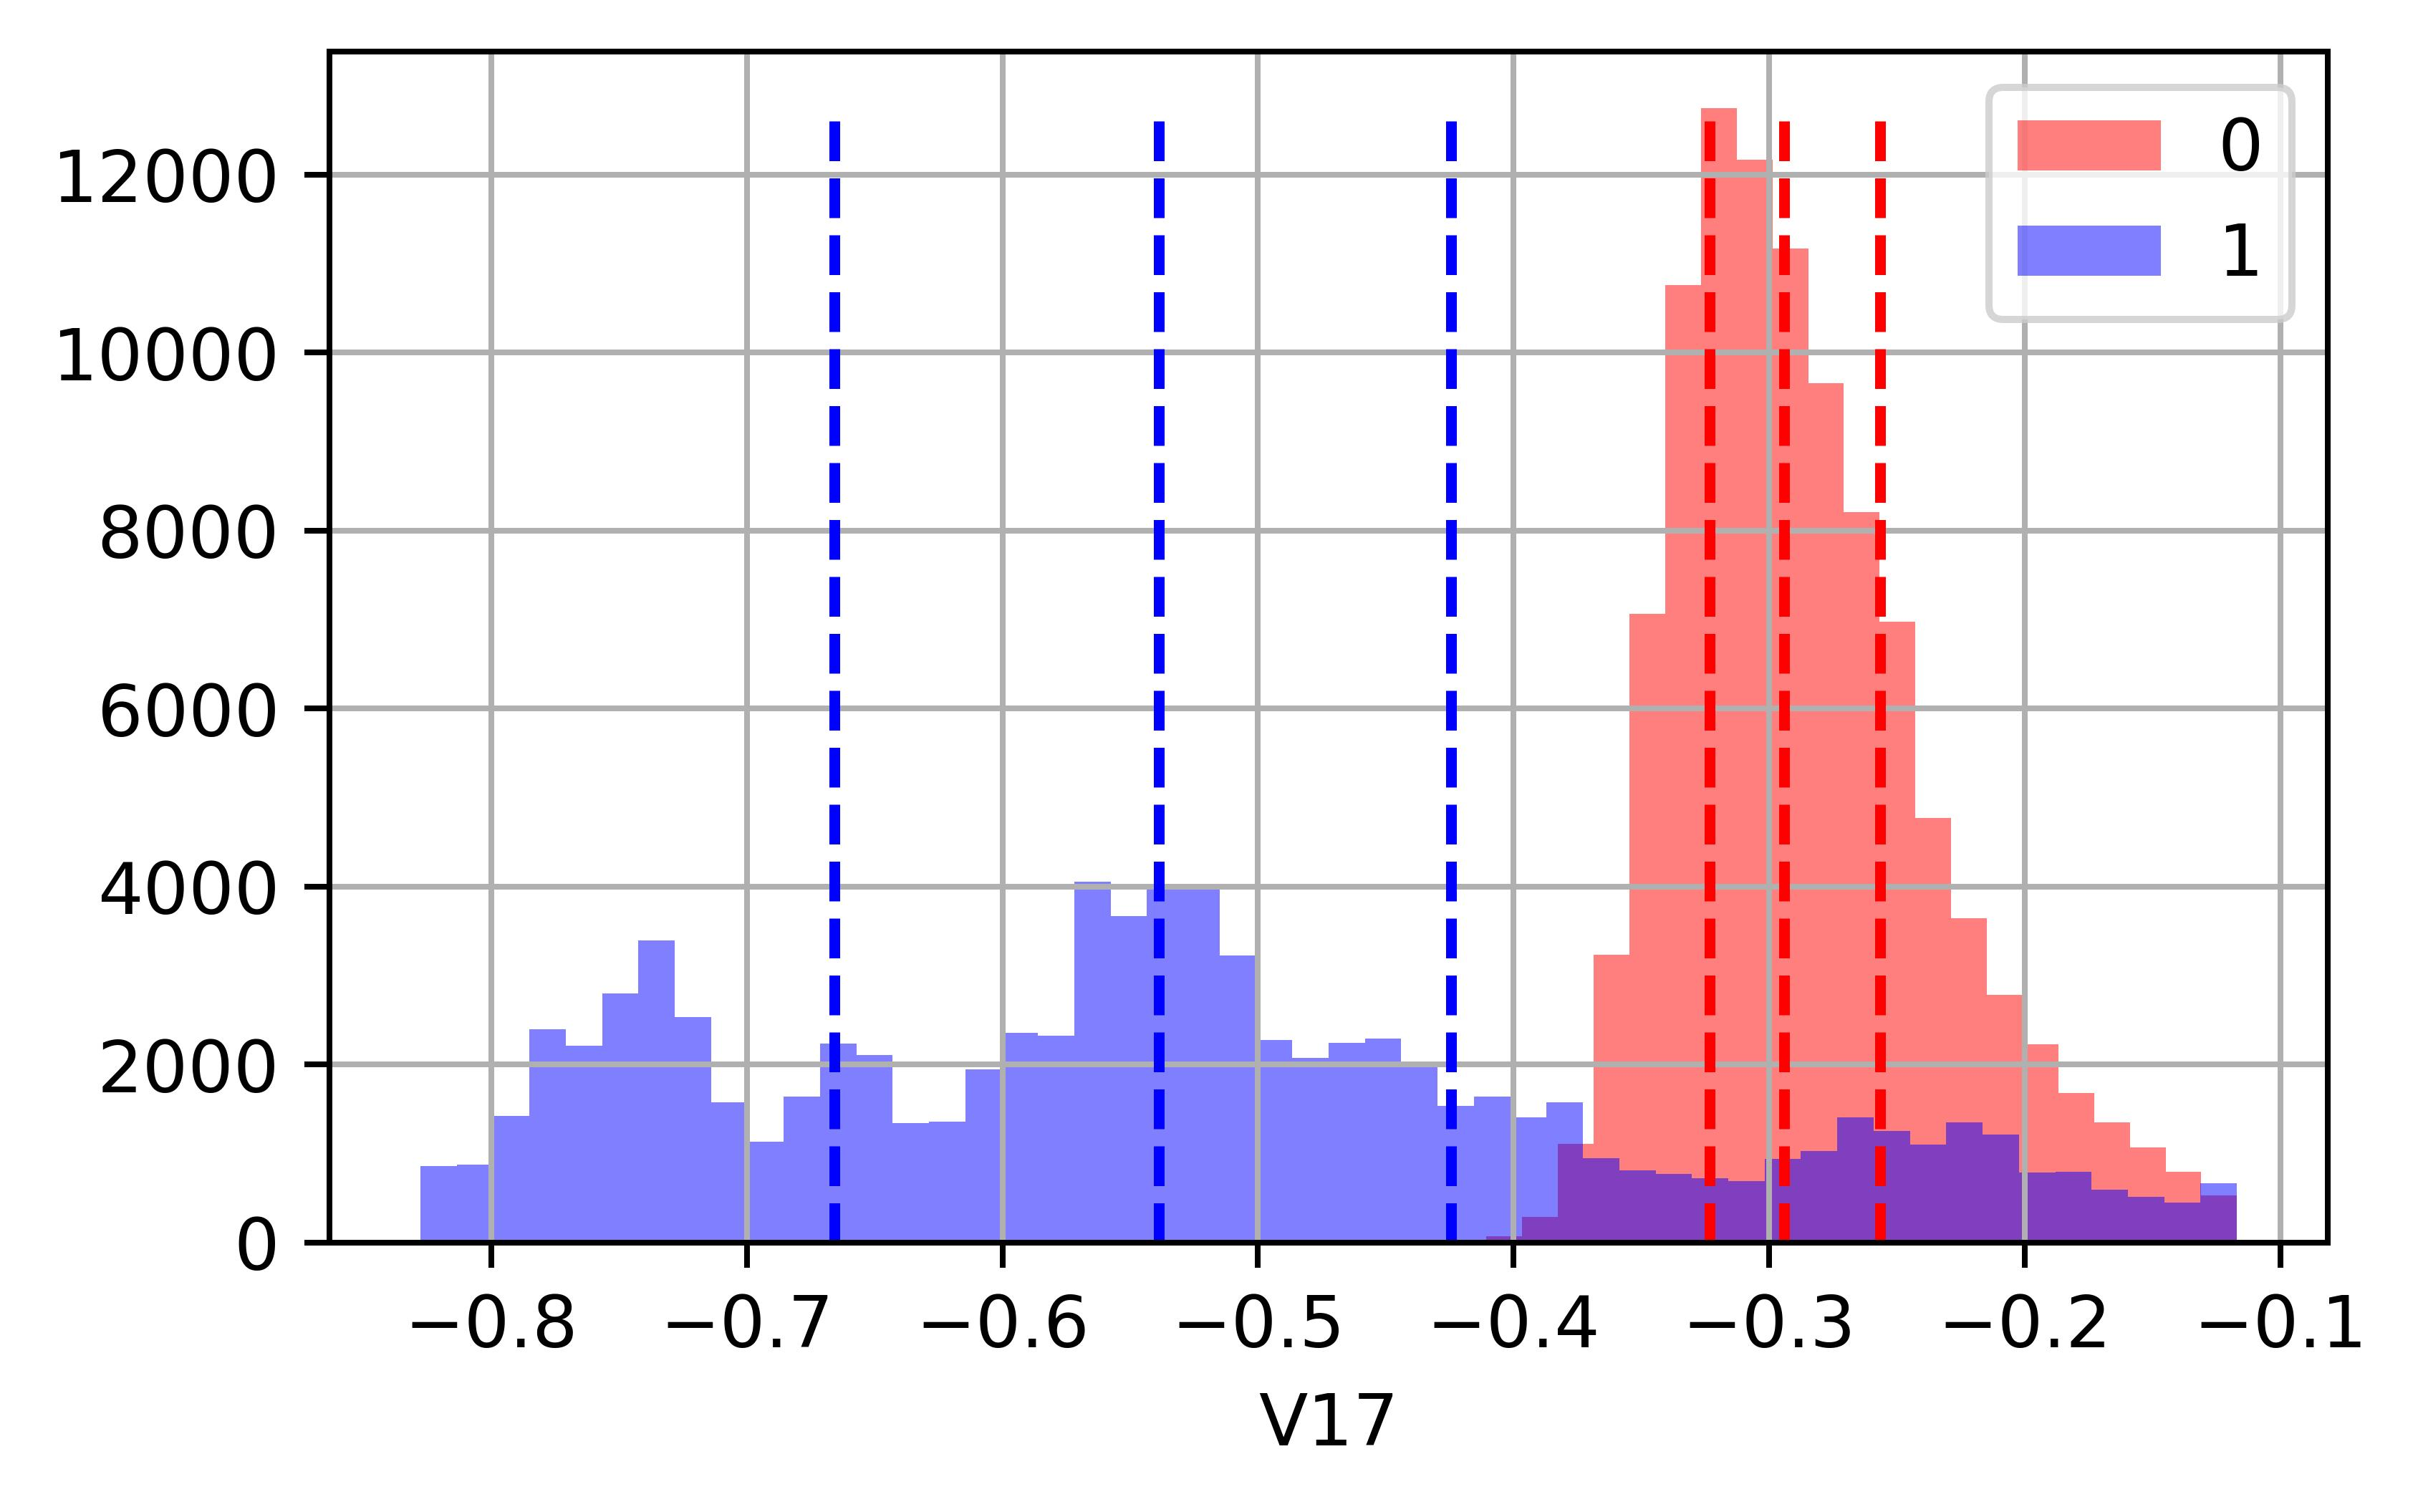
\includegraphics[width=0.3\textwidth]{../code/Task3/Analysis/Hist-16.jpg}
    \caption{Data visualization for task 3. The top shows the parallel coordinate plot for each features (we chose $10\%$ of total data), and the below shows some features that can be linearly separable (the top and bottom $5\%$ points are considered as outliers, and will not be shown).}
  \end{figure}

\end{frame}

\begin{frame}{Task 3 - Correlation Coefficient}

  \begin{figure}[H]
    \centering
    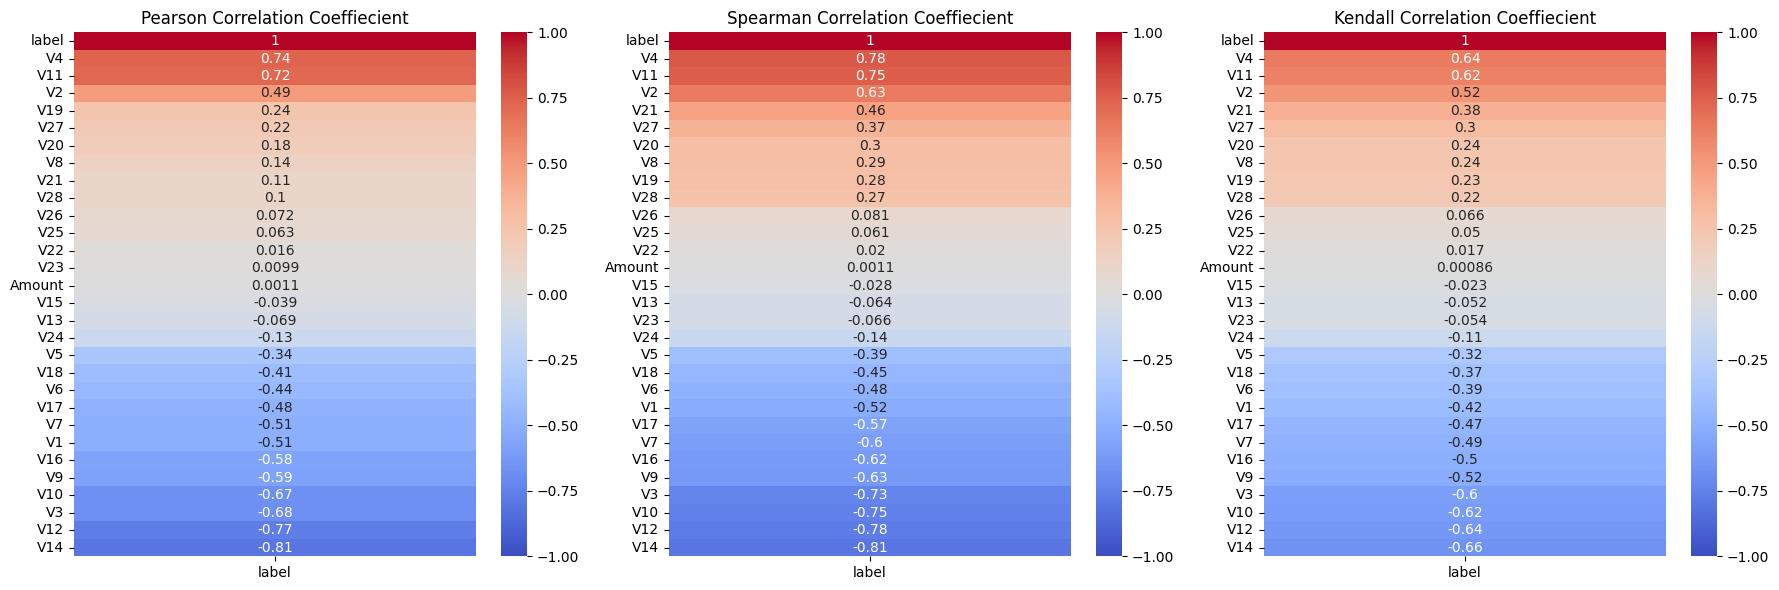
\includegraphics[width=\textwidth]{../code/Task3/Analysis/corrcoef.jpg} \\
    \caption{Correlation coefficient for each features.}
  \end{figure}

  We droped the features with all the correlation coefficient less than a threshold (e.g. 0.1).

\end{frame}

\begin{frame}{Task 3 - Preformance - Logistic Regression}

  \begin{table}[H]
    \centering
    \begin{tabular}{|c|c|c|c|c|}
      \hline
      Penalty & \makecell{Dimension                                 \\ Raising \\ (Degree)} & \makecell{Feature \\ Selection} & F1 Score & \makecell{Time/Mem \\ (s/MB)} \\
      \hline
      None    & None                & False & $0.9586$ & $19.5/866$ \\
      \hline
      None    & $2$                 & False & $0.9619$ & $33.5/915$ \\
      \hline
      None    & $3$                 & False & $0.9621$ & $49.6/973$ \\
      \hline
      Lasso   & None                & False & $0.9579$ & $21.5/854$ \\
      \hline
      Ridge   & None                & False & $0.9553$ & $19.8/853$ \\
      \hline
      None    & None                & True  & $0.9582$ & $16.5/825$ \\
      \hline
    \end{tabular}
    \caption{Preformance for logistic regression. We tested each option with $5$ times cross validation ($80\%$ for training set, $20\%$ for training set) and $1$ times that using all data as training set. The f1 scores showed in the table is the average f1 score for cross validation, the time is the total time for $6$ run, and the memory usage is tested using all the data as training set.}
  \end{table}

\end{frame}

\begin{frame}{Task 3 - Preformance - MLP}

  \begin{table}[H]
    \centering
    \begin{tabular}{|c|c|c|c|c|}
      \hline
      Dropout & Hidden Size & \makecell{Feature                         \\ Selection} & F1 Score & \makecell{Time/Mem \\ (s/MB)} \\
      \hline
      $0.1$   & $32$        & False             & $0.9522$ & $31.9/929$ \\
      \hline
      $0.2$   & $32$        & False             & $0.9000$ & $31.1/916$ \\
      \hline
      $0.1$   & $32$        & True              & $0.9481$ & $31.3/899$ \\
      \hline
      $0.1$   & $16$        & False             & $0.9503$ & $31.7/929$ \\
      \hline
      $0.1$   & $64$        & True              & $0.9500$ & $29.7/902$ \\
      \hline
    \end{tabular}
    \caption{Preformance for MLP. We tested each option with $5$ times cross validation ($80\%$ for training set, $20\%$ for training set) and $1$ times that using all data as training set. The f1 scores showed in the table is the average f1 score for cross validation, the time is the total time for $6$ run, and the memory usage is tested using all the data as training set.}
  \end{table}

\end{frame}

\section{Summary}

\begin{frame}{Summary}

  \begin{itemize}
    \item Well designed feature engineering, including feature selection and dimension raising, can lead to a better model performance; \vspace{.25cm}
    \item The decision tree will be more prone to overfitting the data; \vspace{.25cm}
    \item The MLP can handle both linear and nonlinear data, but it is sensitive to hyperparameters. \vspace{.25cm}
  \end{itemize}

\end{frame}

\section*{Reference}
\begin{frame}[allowframebreaks]{Reference}
  \printbibliography
\end{frame}

\appendix

\end{document}